\documentclass[12pt]{witseiepaper}
\usepackage{KJN}
\usepackage[a4paper,top=25mm, bottom=32mm, left=20mm, right=20mm]{geometry}
\usepackage{pdfpages}
% Set the page size to be A4 as opposed to the default US Letter
\usepackage{graphicx} 

% Required for including pictures
\usepackage{float} 


\usepackage{wrapfig} 
\usepackage{array,booktabs}% http://ctan.org/pkg/{array,booktabs}
%%%%%%%%%%%%%%%
\usepackage{fancyhdr}
\usepackage{pdfpages}

\pagestyle{fancy}
\fancyhf{}
\fancyfoot[C]{\thepage}

\ifpdf
\pdfinfo{
% /Title (INSTRUCTIONS AND STYLE GUIDELINES FOR THE PREPARATION OF FINAL YEAR LABORATORY PROJECT PAPERS : 2005 VERSION)
% /Author (Ken J Nixon)
% /CreationDate (D:200309251200)
% /ModDate (D:200510121530)
% /Subject (ELEN417/455 Paper Format, 2005)
% /Keywords (ELEN417, ELEN455, paper, instructions, style guidelines, laboratory project)
}
\fi

%%%%%%%%%%%%%%%%%%%%%%%%%%%%%%%%%%%%%%%%%%%%%%%%%%%%%%%%%%%%%%%%%%%%%%%%%%%%%%%

\begin{document}


%----------------------------------------------------------------------------------------
% TITLE PAGE
%----------------------------------------------------------------------------------------
\begin{titlepage}
  
  \newcommand{\HRule}{\rule{\linewidth}{0.5mm}} 
  
  % Defines a new command for the horizontal lines, change thickness here
  \begin{center}
    
    % Center everythingn the page
    \textsc{\LARGE ELEN7046}\\[1.5cm]
    
    % Name of your university/college
    \textsc{\Large University of Witwatersrand}\\[0.5cm]
    
    % Major heading such as course name
    \textsc{\large Software Technologies and Techniques}\\[0.5cm]
    
    % Minor heading such as course title
    \HRule \\[0.4cm]
    { \huge \bfseries Group Project Report: SirVey}\\[0.5cm]
    
    % Title of your document
    \HRule \\[1.5cm]
    \begin{minipage}
      {0.4
      \textwidth} 
      \begin{flushleft}
        \large \emph{Authors:}\\
        Avanindra (Avy) \textsc{Singh} \\
        Leslie \textsc{Dobrowsky} \\
        Lishen \textsc{Ramsudh} \\
        Peter \textsc{Cousins} \\
        Bakwanyana \textsc{Thobela} \\
        
        % Your name
      \end{flushleft}
    \end{minipage}
    ~ 
    \begin{minipage}
      {0.4
      \textwidth} 
      \begin{flushright}
        \large \emph{Student Number:} \\
        0704012 \textsc{N} \\
        9409714 \textsc{M}  \\
        1312875 \\
        782377  \\
        855470
        % Supervisor's Name
      \end{flushright}
    \end{minipage}
    \\[2cm]
    
    {\large \today}\\[2cm]
    
    % Date, change the \today to a set date if you want to be precise
  \end{center}
  \large

 % \textbf{Abstract}  \\[0.1cm]
 %  This document focuses on mock objects. It defines mock objects as a technique in software development commonly used in unit testing. A brief list of when to use mock objects is presented. The differences and a clear definition of each type of ``simulated object'' is given for dummy objects, fake objects, stub objects and mock objects. Mock objects insist on behaviour verification as opposed to other types of objects which usually are state verification. A practical example is illustrated using EasyMock in Java. The application of mock objects in unit testing is then discussed. It is concluded that using mock objects can be a advantage or disadvantage depending on the context of the system under test.

  \textbf{}
  % Dummy text
  %\end{flushleft}
  %\includegraphics{Logo}\\[1cm] % Include a department/university logo - this will require the graphicx package
  %\vfill % Fill the rest of the page with whitespace
\end{titlepage}


% \title{INSTRUCTIONS AND STYLE GUIDELINES FOR THE PREPARATION OF FINAL YEAR LABORATORY PROJECT PAPERS : 2005 VERSION}

% \author{Ken J. Nixon
% \thanks{School of Electrical \& Information Engineering, University of the
% Witwatersrand, Private Bag 3, 2050, Johannesburg, South Africa}
% }

%%%%%%%%%%%%%%%%%%%%%%%%%%%%%%%%%%%%%%%%%%%%%%%%%%%%%%%%%%%%%%%%%%%%%%%%%%%%%%%
%%%%%%%%%%%%%%%%%%%%%%%%%%%%%%%%%%%%%%%%%%%%%%%%%%%%%%%%%%%%%%%%%%%%%%%%%%%%%%%
%%%%%%%%%%%%%%%%%%%%%%%%%%%%%%%%%%%%%%%%%%%%%%%%%%%%%%%%%%%%%%%%%%%%%%%%%%%%%%%'

 \thispagestyle{empty}\pagestyle{empty}
 \begin{center}
  \textsc{\bfseries APPLICATION DETAILS} \\ [1.0cm]
 \end{center}


  \textbf{Application Name:} \textsc{SirVey} \\
   \\
   \textbf{\textsc{Source Code Repositories:}}\\
   \\
	https://github.com/ReddragonLR/ELEN7046ServerAndAdmin.git \\
	https://github.com/ReddragonLR/ELEN7046AndroidApp/tree/master/SirVey \\

\textbf{This Repositories contain the following projects:}
\begin{itemize}
\item An MS Access based solution
\item A java web page solution
\item A web-based survey using Ruby as a back-end and AngularJS as the front-end
\item A web-based survey using the MEAN stack. Requirements:
\item The Android Mobile Application
\end{itemize}

% Signed:\\
% \rule[1em]{25em}{0.5pt} % This prints a line for the signature
%  \\ [1.5cm]
% Date:\\
% \rule[1em]{25em}{0.5pt} % This prints a line to write the date

\clearpage % Start a new page
%----------------------------------------------------------------------------------------
% DECLARATION PAGE
% Your institution may give you a different text to place here
%----------------------------------------------------------------------------------------
 % \renewcommand\thesection{\Alph{section}}
 % \setcounter{section}{0}

 \thispagestyle{empty}\pagestyle{empty}
 
 \newpage
 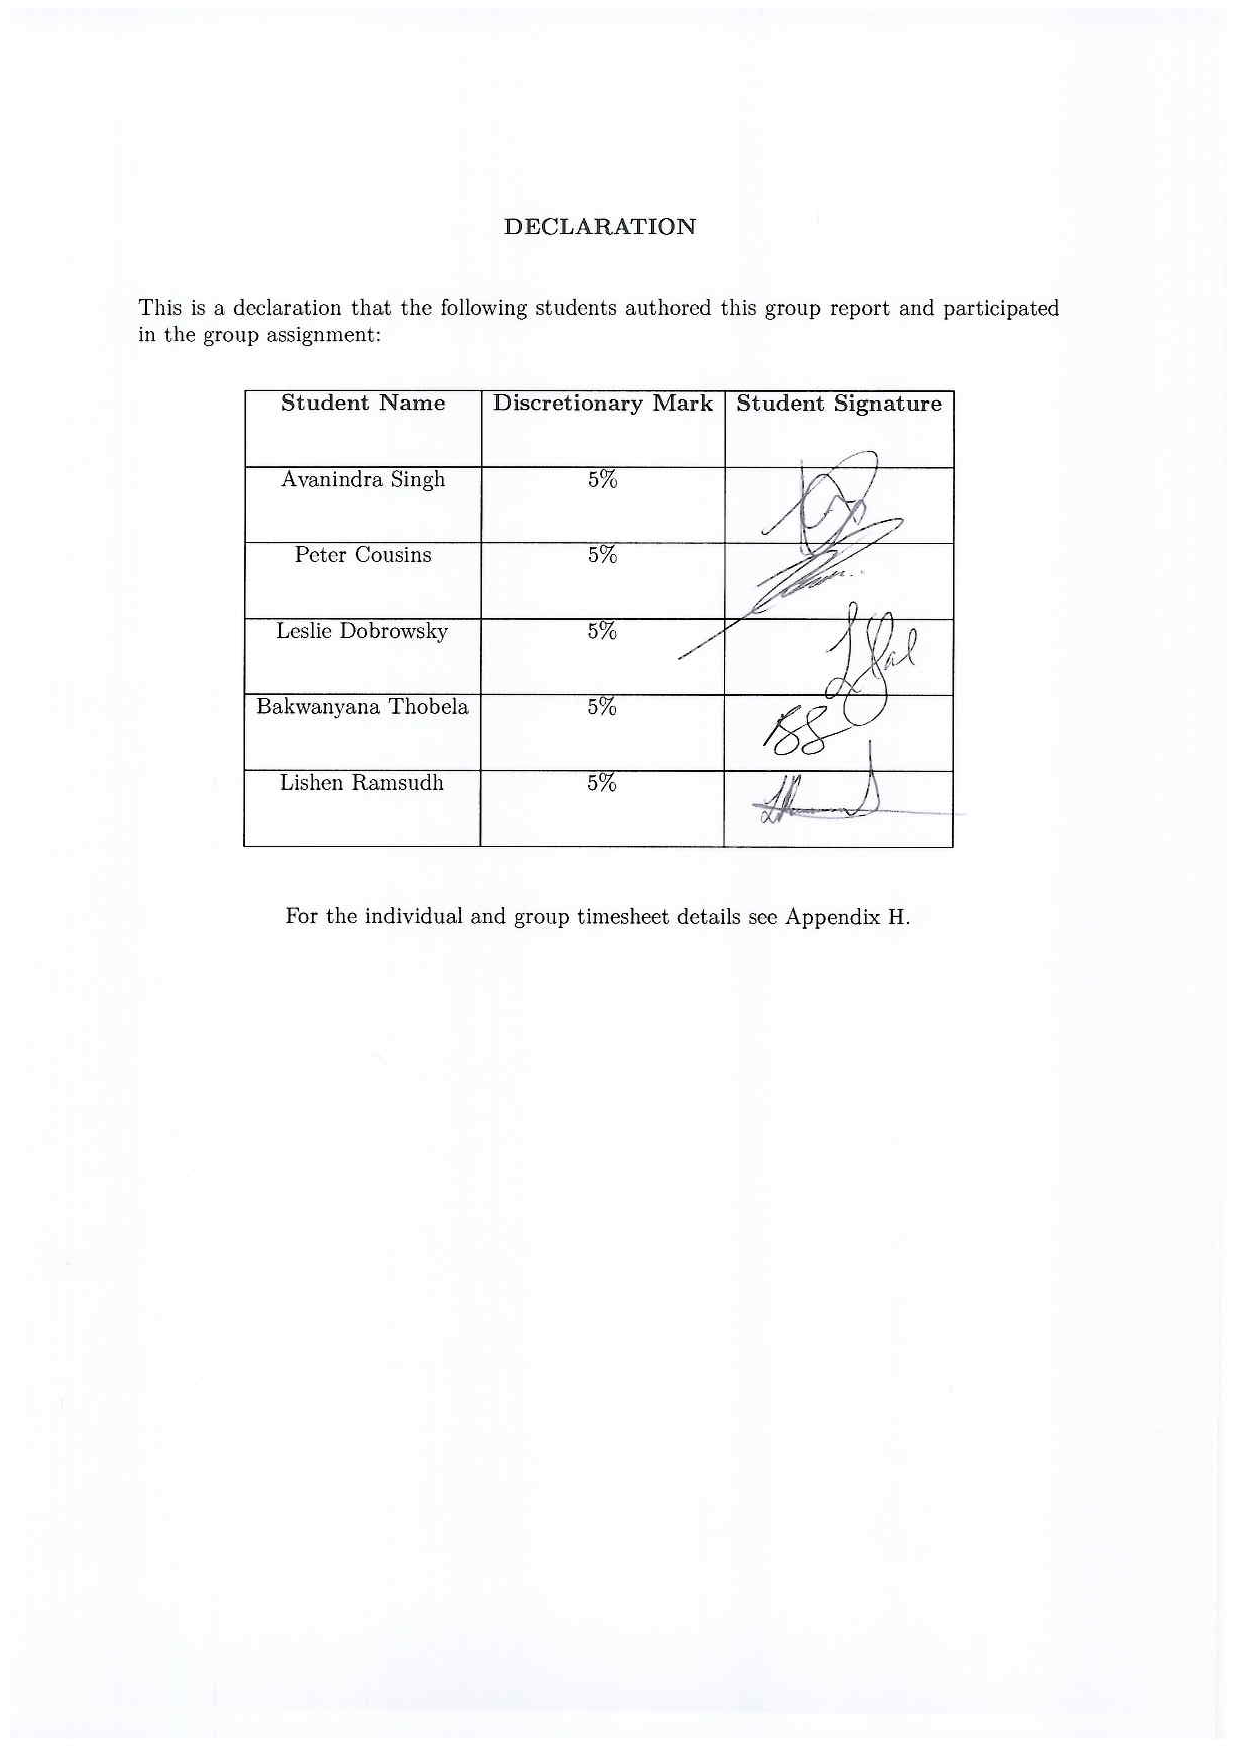
\includepdf[pages=1]{./Guides/CPDSign.pdf}
 
 

% I ALTER THIS TO PLEDGEARISM AND GROUP WORK BREAKDOWN, Avanindra Singh, declare that this thesis titled, 'My Thesis' and the work presented in it are my own. I confirm that:

% \begin{itemize} 
% \item This work was done wholly or mainly while in candidature for a research degree at this University. \\
% \item Where any part of this thesis has previously been submitted for a degree or any other qualification at this University or any other institution, this has been clearly stated. \\
% \item Where I have consulted the published work of others, this is always clearly attributed. \\
% \item Where I have quoted from the work of others, the source is always given. With the exception of such quotations, this thesis is entirely my own work. \\
% \item I have acknowledged all main sources of help. \\
% \item Where the thesis is based on work done by myself jointly with others, I have made clear exactly what was done by others and what I have contributed myself.\\ [1.5cm]
% \end{itemize}

% Signed:\\
% \rule[1em]{25em}{0.5pt} % This prints a line for the signature
%  \\ [1.5cm]
% Date:\\
% \rule[1em]{25em}{0.5pt} % This prints a line to write the date



\clearpage % Start a new page

%%%%%%%%%%%%%%%%%%%%%%%%%%%%%%%%%%%%%%%%%%%%%%%%%%%%%%%%%%%%%%%%%%%%%%%%%%%%%%%
%%%%%%%%%%%%%%%%%%%%%%%%%%%%%%%%%%%%%%%%%%%%%%%%%%%%%%%%%%%%%%%%%%%%%%%%%%%%%%%
%%%%%%%%%%%%%%%%%%%%%%%%%%%%%%%%%%%%%%%%%%%%%%%%%%%%%%%%%%%%%%%%%%%%%%%%%%%%%%%

%----------------------------------------------------------------------------------------
% QUOTATION PAGE
%----------------------------------------------------------------------------------------

% \pagestyle{empty} % No headers or footers for the following pages

% \null\vfill % Add some space to move the quote down the page a bit

% \textit{``Thanks to my solid academic training, today I can write hundreds of words on virtually any topic without possessing a shred of information, which is how I got a good job in journalism."}

% \begin{flushright}
% Dave Barry
% \end{flushright}

% \vfill\vfill\vfill\vfill\vfill\vfill\null % Add some space at the bottom to position the quote just right

% \clearpage % Start a new page


%%%%%%%%%%%%%%%%%%%%%%%%%%%%%%%%%%%%%%%%%%%%%%%%%%%%%%%%%%%%%%%%%%%%%%%%%%%%%%%
%%%%%%%%%%%%%%%%%%%%%%%%%%%%%%%%%%%%%%%%%%%%%%%%%%%%%%%%%%%%%%%%%%%%%%%%%%%%%%%
%%%%%%%%%%%%%%%%%%%%%%%%%%%%%%%%%%%%%%%%%%%%%%%%%%%%%%%%%%%%%%%%%%%%%%%%%%%%%%%
%%%%%%%%%%%%%%%%%%%%%%%%%%%%%%%%%%%%%%%%%%%%%%%%%%%%%%%%%%%%%%%%%%%%%%%%%%%%%%%
%%%%%%%%%%%%%%%%%%%%%%%%%%%%%%%%%%%%%%%%%%%%%%%%%%%%%%%%%%%%%%%%%%%%%%%%%%%%%%%
%%%%%%%%%%%%%%%%%%%%%%%%%%%%%%%%%%%%%%%%%%%%%%%%%%%%%%%%%%%%%%%%%%%%%%%%%%%%%%%
 \thispagestyle{empty}\pagestyle{empty}
 \begin{center}
  \textsc{\bfseries ABSTRACT} \\ [1.0cm]
  % \section{ABSTRACT}
  \end{center}
  This document focuses on mock objects. It defines mock objects as a technique in software development commonly used in unit testing. A brief list of when to use mock objects is presented. The differences and a clear definition of each type of ``simulated object'' is given for dummy objects, fake objects, stub objects and mock objects. Mock objects insist on behaviour verification as opposed to other types of objects which usually are state verification. A practical example is illustrated using EasyMock in Java. The application of mock objects in unit testing is then discussed. It is concluded that using mock objects can be a advantage or disadvantage depending on the context of the system under test.
 \\

{\bfseries Key Words: } Software Prototype, Survey, SCRUM .\\ [1.0cm]
% %


\keywords{Four to six key words in alphabetical order, separated by commas.}

\clearpage % Start a new page
%%%%%%%%%%%%%%%%%%%%%%%%%%%%%%%%%%%%%%%%%%%%%%%%%%%%%%%%%%%%%%%%%%%%%%%%%%%%%%%
%%%%%%%%%%%%%%%%%%%%%%%%%%%%%%%%%%%%%%%%%%%%%%%%%%%%%%%%%%%%%%%%%%%%%%%%%%%%%%%
% %%%%%%%%%%%%%%%%%%%%%%%%%%%%%%%%%%%%%%%%%%%%%%%%%%%%%%%%%%%%%%%%%%%%%%%%%%%%%%%
%  \thispagestyle{empty}\pagestyle{empty}
%  \begin{center}
%  % \textsc{\bfseries ACKNOWLEDGEMENTS} \\ [1.0cm]
%  \section{ACKNOWLEDGEMENTS}
%  \end{center}
% The acknowledgements and the people to thank go here, don't forget to include your project advisor.
% The preferred spelling of the word ``acknowledgement'' in British English is
% with an ``e'' after the ``g.'' Use the singular heading even if you have
% several acknowledgements. Use this section for sponsor and financial support
% acknowledgments. This is also an ideal section to acknowledge the
% contribution made by your fellow group member.

% The authors would like to acknowledge the Department of Electronic and
% Electrical Engineering at the University of Sheffield for the use of their
% paper template for the LDIA2003 symposium proceedings as well as the South
% African Institute of Electrical Engineers for parts of the style guidelines
% for publications in the SAIEE transactions.  Additional thanks are extended to
% Andr\'e van Zyl and Steve Levitt for their invaluable contributions.




% \clearpage % Start a new page

% %%%%%%%%%%%%%%%%%%%%%%%%%%%%%%%%%%%%%%%%%%%%%%%%%%%%%%%%%%%%%%%%%%%%%%%%%%%%%%%





%%%%%%%%%%%%%%%%%%%%%%%%%%%%%%%%%%%%%%%%%%%%%%%%%%%%%%%%%%%%%%%%%%%%%%%%%%%%%%%
%%%%%%%%%%%%%%%%%%%%%%%%%%%%%%%%%%%%%%%%%%%%%%%%%%%%%%%%%%%%%%%%%%%%%%%%%%%%%%%
%%%%%%%%%%%%%%%%%%%%%%%%%%%%%%%%%%%%%%%%%%%%%%%%%%%%%%%%%%%%%%%%%%%%%%%%%%%%%%%
%%%%%%%%%%%%%%%%%%%%%%%%%%%%%%%%%%%%%%%%%%%%%%%%%%%%%%%%%%%%%%%%%%%%%%%%%%%%%%%
%%%%%%%%%%%%%%%%%%%%%%%%%%%%%%%%%%%%%%%%%%%%%%%%%%%%%%%%%%%%%%%%%%%%%%%%%%%%%%%
%%%%%%%%%%%%%%%%%%%%%%%%%%%%%%%%%%%%%%%%%%%%%%%%%%%%%%%%%%%%%%%%%%%%%%%%%%%%%%%




%%%%%%%%%%%%%%%%%%%%%%%%%%%%%%%%%%%%%%%%%%%%%%%%%%%%%%%%%%%%%%%%%%%%%%%%%%%%%%%
%%%%%%%%%%%%%%%%%%%%%%%%%%%%%%%%%%%%%%%%%%%%%%%%%%%%%%%%%%%%%%%%%%%%%%%%%%%%%%%
%%%%%%%%%%%%%%%%%%%%%%%%%%%%%%%%%%%%%%%%%%%%%%%%%%%%%%%%%%%%%%%%%%%%%%%%%%%%%%%
% %%%%%%%%%%%%%%%%%%%%%%%%%%%%%%%%%%%%%%%%%%%%%%%%%%%%%%%%%%%%%%%%%%%%%%%%%%%%%%%




%%%%%%%%%%%%%%%%%%%%%%%%%%%%%%%%%%%%%%%%%%%%%%%%%%%%%%%%%%%%%%%%%%%%%%%%%%%%%%%
%%%%%%%%%%%%%%%%%%%%%%%%%%%%%%%%%%%%%%%%%%%%%%%%%%%%%%%%%%%%%%%%%%%%%%%%%%%%%%%
%%%%%%%%%%%%%%%%%%%%%%%%%%%%%%%%%%%%%%%%%%%%%%%%%%%%%%%%%%%%%%%%%%%%%%%%%%%%%%%
%%%%%%%%%%%%%%%%%%%%%%%%%%%%%%%%%%%%%%%%%%%%%%%%%%%%%%%%%%%%%%%%%%%%%%%%%%%%%%%
%%%%%%%%%%%%%%%%%%%%%%%%%%%%%%%%%%%%%%%%%%%%%%%%%%%%%%%%%%%%%%%%%%%%%%%%%%%%%%%
%%%%%%%%%%%%%%%%%%%%%%%%%%%%%%%%%%%%%%%%%%%%%%%%%%%%%%%%%%%%%%%%%%%%%%%%%%%%%%%




%%%%%%%%%%%%%%%%%%%%%%%%%%%%%%%%%%%%%%%%%%%%%%%%%%%%%%%%%%%%%%%%%%%%%%%%%%%%%%%
%%%%%%%%%%%%%%%%%%%%%%%%%%%%%%%%%%%%%%%%%%%%%%%%%%%%%%%%%%%%%%%%%%%%%%%%%%%%%%%
%%%%%%%%%%%%%%%%%%%%%%%%%%%%%%%%%%%%%%%%%%%%%%%%%%%%%%%%%%%%%%%%%%%%%%%%%%%%%%%
% %%%%%%%%%%%%%%%%%%%%%%%%%%%%%%%%%%%%%%%%%%%%%%%%%%%%%%%%%%%%%%%%%%%%%%%%%%%%%%%
% %
% \abstract{The purpose of this document is to provide an easy-to-use
% template/style sheet to enable authors to prepare papers in the correct format
% and style for the final year laboratory project. This document may be
% downloaded from the School of Electrical and Information Engineering web site
% and can be used as a template. To ensure conformity of appearance it is
% essential that these instructions are followed. The abstract should be limited
% to 50-200 words, which should concisely summarise the paper.}

% \keywords{Four to six key words in alphabetical order, separated by commas.}


% \maketitle
% \thispagestyle{empty}\pagestyle{empty}
\pagestyle{plain}

\pagenumbering{roman}

\tableofcontents
% test\index{test}

\newpage
\listoffigures % Write out the List of Figures
\newpage
\listoftables % Write out the List of Tables
\newpage
\renewcommand\thesection{\arabic{section}}
\renewcommand\thesubsection{\thesection.\arabic{subsection}}
 \setcounter{section}{0}
\pagenumbering{arabic}
\setcounter{page}{1}
%%%%%%%%%%%%%%%%%%%%%%%%%%%%%%%%%%%%%%%%%%%%%%%%%%%%%%%%%%%%%%%%%%%%%%%%%%%%%%%
%
\section{Introduction}

In South Africa there are many services such as electricity, water and healthcare which are freely available to citizens or at low cost. The distribution of these basic resources could be defined as "service delivery". It has been publicised in media that healthcare service delivery has an impact on millions of peoples lives including their mortality \cite{InfantsDie}. Obtaining feedback on the health care system is critical to improving all citizens experiences of the health care system.

The purpose of this project is to produce a means to obtain feedback from local and remote communities utilising the health care systems, specifically through developing a software application which can be used to conduct surveys. By conducting surveys efficiently and through a software application data can be obtained and analysed to provide appropriate reporting on how efficient the service delivery of health care in a particular area. South Africa as a third world country faces unique challenges such as connectivity to the internet \cite{Internet} which imposes challenges from a application development point of view. 

To conduct surveys and collect feed back from any citizen who utilises any service in healthcare will greatly assist both the communities as well as government officials. A project team was assembled and tasked with producing a proof of concept (POC) of the survey software application. This report documents the project team's approach in terms of the team organisation, methodology adopted, design decisions and the engineering trade-off considerations in producing the final solution.

\subsection{Project Requirements}

The purpose of this project is to design a software application which will be used to gather information on the public health care service delivery and provide appropriate reporting. The surveys will be conducted in areas with little internet connectivity. This means that application must cater for capturing data "offline" and then uploaded centrally for reporting.\\

\section{Literature Review}
\subsection{Existing Solutions}

There are a large number of solutions that exist in the market in terms of software applications which can be used to conduct surveys. Some of the solutions on the market do satisfy the basic project requirements \cite{ReviewSurvey}. SurveyGizmo \cite{SurveyGizmo} is a web application (software as a service) platform which features 28 different customizable possible survey question and answer combinations. This solution satisfies all requirements in particular the off-line capability, custom reporting and developer integration. SurveyMonkey \cite{SurveyMonkey} is similar to SurveyGizmo in that it offers a similar feature set. It also offers the ability to create custom reporting with text analysis. SurveyMonkey also features telephonic surveys where users are able to create surveys and have respondents answer using voice. 

\subsection{Standards, Regulations and Policy}
Depending on the information that is captured through survey questions there could be standards, regulations and policies which need to be adhered to. An example of this would be in the health care sector where the Act of 1996 (HIPAA) could be applied. The Act of 1996 (HIPAA) is a set of rules to be followed by health plans, doctors, hospitals and other health care providers \cite{HIPAA}. It is essential to adopt the standards for electronic health care transactions and identifiers for providers, health plans, and employers. To date, the implementation of HIPAA standards has increased the use of electronic data interchange \cite{HIPAA}. HIPAA also contains a privacy rule which protects any data gathered from patients in the health care environment. Therefore to comply with HIPAA it essential for any software to have security so that patients are not compromised in terms of the act. Software should comply completely with HIPAA if it is to be used in a health service delivery environment. \\

\section{Project Framework} 

\subsection{Business Case} 
  
\noindent By conducting surveys, one can identify the misalignment between services required by communities and services rendered by its designated service providers. The result of gathering information about service delivery (in this scenario specifically health care) is that insights and observations can be gained in order to improve service delivery. This could have a variety of impacts including improving people's ability to receive high levels of service and possibly have an impact on their quality of life. Increasing the amount of engagement with the community allows for feedback to be provided to improve service delivery.

\subsection{Scope of the Application}
The scope of the application progressively changes with each iteration. As an iteration is successful more features and improvements can be added to each version of the project.

\emph{Key Users} 
\begin{itemize}
  \item \textbf{Surveyors:} These are the individuals who will utilise the application to capture surveys and get responses from the community.
  \item \textbf{Administrators:} These are the business owners who define questions and will create surveys and utilise the reporting features of the application to gain insights from the communities responses.
\end{itemize}

\emph{Stakeholders} 
\begin{itemize}
  \item \textbf{Community:} These are the actual people who utilise services and who will provide feedback on the service delivery through the survey project. The community by voicing their concerns and opinions will enjoy improved services (e.g. health care) provided by the service provider based on the feedback gathered.
  \item \textbf{Application Administrators:} Provide administrator services, maintenance and creation of surveys.
  \item \textbf{Surveyors:} Users who conduct surveys through the platform.
  \item \textbf{Development Team:} Responsible for creating and maintaining the platform. 
\end{itemize}


\subsection{Project Requirements}
\subsubsection{Specification By Example}
Specification by Example (SBE) is a collaborative approach whereby the team defines requirements and business orientated functional tests for software based on capturing and illustrating requirements using realistic examples \cite{SBE}. This method is utilised to obtain the specific requirements of the project.
Table ~\ref{tbl:use} shows a list of the specifications by example that are applicable to the project. Appendix A features the detailed requirement specifications artefacts including key examples as well as the specifications by example.

\begin{table}[htb] \caption{Table showing a list of the key examples.} \label{tbl:use} 
    \begin{center}
  \begin{tabular}
    {|c|c|} \hline \textbf{Use} &\textbf{Description}\\
    \textbf{Case} &\\
    \hline 1 &Conducting a Survey\\
    \hline 2 &Reporting\\
    \hline 3 &Offline Mode\\
    \hline 4 &Survey Administration\\
    \hline 5 &User Access\\
    \hline 
  \end{tabular}
      \end{center}
\end{table}

\subsection{Project Constraints}
\begin{itemize}
  \item The project has a time constraint. 
  \item The project does not have unlimited software development resources and each member of the team has different skills. 
  \item The project should be intellectually challenging and must allow for each member of the team to learn new tools, techniques and programming skills.
  \item The project must contain 25\% original source code.
  \item The project solution must be able to function in an environment with little or no connectivity.
\end{itemize}

\subsection{Project Assumptions}
\begin{itemize}
  \item The users specifically the surveyors are honest and do complete surveys and do not fraudulently answer the surveys themselves.
  \item The surveyors do not necessarily have internet connectivity when doing surveys in the community.
  \item The surveyors have the equipment and resources necessary to utilise the project solution in order to conduct surveys in the community.
  \item The data is uploaded to a central point for analysis and reporting. This means that it is not required to generate reporting at the point of surveying.
\end{itemize}


\subsection{Success Criteria}
\subsubsection{For the users}
\begin{itemize}
  \item Surveyors \begin{itemize}
  \item Surveyors are able to capture answers in the form of yes/no questions, free form text and a selection with predefined answers.
  \end{itemize}
    \item Administrators \begin{itemize}
  \item Administrators should be able to create any surveys with the desired answer options.
  \item They should be able to authenticate and login in to the platform.
  \item Administrators should be able to view reporting information on the surveys which have successfully uploaded to the system.
  \end{itemize}

\end{itemize}

\subsubsection{For the project}
\begin{itemize}
  \item The solution must be able to capture surveys in a off-line mode with the ability to upload to a central point for reporting.
  \item Be able to capture surveys on multiple channels and multiple devices.
  \item The device of choice preferably being Android should support as many devices as possible.
  \item Analytics of the data should be centralised.
  \item Surveys are dynamic and can be refreshed in field (given internet connectivity).
  \item There is no custom configuration necessary on any device that the surveyors utilise. This means they can be provisioned in-field.
  \item The system can handle multiple surveyors in the field gathering responses.
  \item The system can also handle multiple types of surveys.
  \item Training guides and development guides should be documented.
\end{itemize}

\subsection{Licensing Requirements}
This project should utilise MIT licenses and free licences where possible.

\section{Project Execution}
A software project's successful execution relies heavily on the project team meeting all desired success criteria defined in the project requirements. To make sure the project team remains on track a specially role is required within the project team, this is commonly known as a software project manager (PM). \cite{SPM}

The project manager role is to manage all of the organizing and planning of a project. This may entail formalizing task allocation and tracking the estimated effort vs. the actual effort expended.
While tracking the team’s effort the budget and cost analysis also needs to be considered as business stakeholders will require the PM to report back on progress vs. project budget spent. \cite{ExpertJudgement}

The effective communication to all project stakeholders forms part of the project manager’s base responsibilities. Clear and regularly communication of the risks, concerns and progress on a project to the appropriate stakeholders, allows for adjustments and decisions to be made in smaller increments thus allowing the team to adapt and remain on track to achieve the project’s goals.

\subsection{Project Methodology}

Project methodologies in the author's opinion should not be dictated but should rather be discussed and adapted to the projects characteristics. During the first meeting, the team members stated numerous technologies that could achieve the business vision and requirements. However this also lead to scope discussions and possible future scope changes as early as the first planning session.

Due to the highly volatile scope discussions within the team the decision to adopt a crafted quality methodology \cite{craft} started to present itself as a methodology of choice. The project team agreed that the SCRUM methodology \cite{ExpertJudgement} would be implemented and the role of the project manager would change to be a SCRUM master. \cite{SCUMMaster}

\subsection{Project Team}

With the preferred methodology chosen the team formed to take the key roles required to execute the SCRUM methodology. The three primary roles the team required where the SCRUM Master, Product Owner and technical experts.\\

\begin{figure}[H]
	\center{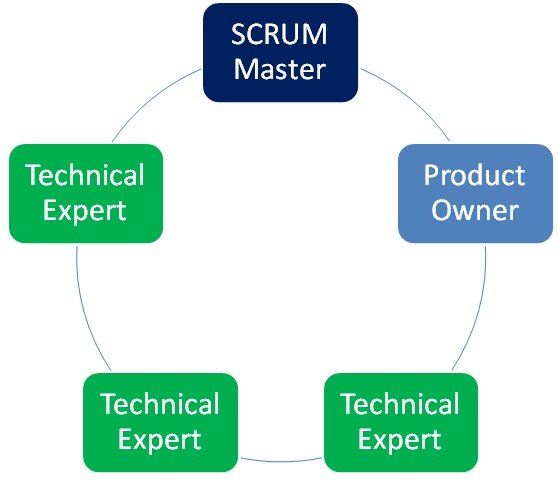
\includegraphics[width=.55\linewidth]{./images/SCRUMTeam}} 
	\caption{SCRUM Team Roles.} 
	\label{fig:SCRUMTeam}
\end{figure}

\subsection{Sprints}

With the project vision and project deadline defined the high level planning allowed for eleven sprints \cite{ExpertJudgement} where one sprint would run for seven days or 75 effort hours. While de-constructing the requirements the high level deliverables were prioritized in the backlog and marked for delivery in specific sprints. The product backlog (PBL) and the detailed sprint planning can be viewed in appendix C. Tracking and reporting on the sprint progress was achieved via a burn down chart \cite{SCUMMaster}. This was created from the project teams timesheets. The burn down chart for the SirVey proof of concept is listed in Appendix K.


\subsection{Project Estimation and Costing}
During the project initiation the business stakeholders will review estimations and high level costing before committing to assigning the budget. \cite{ExpertJudgement} The estimations for the proof of concept (POC) where based on variable scope and requirements. Due to the variability in requirements the estimation accuracy will not be at a high confidence level. Therefore the POC could result in either an over estimation or under estimating. The proof of concept was estimated at a total of 825 effort hours and 5 resources were assigned, the estimation total was produced using an Expert Judgement method \cite{ExpertJudgement}. The team calculated that a single weekly sprint would consist of 75 hours, this would in turn be the project teams weekly burn rate. Therefore if the team assume an average blended resource rate of R 500 an hour the cost per sprint can be calculate as follows.

% MAKE THE TABLE LEFT JUSTIFIED
\begin{table}[htb] \caption{Table showing the effort placed into the project and its cost.} \label{tbl:cost} 
    \begin{center}
  \begin{tabular}
     {|c|c|} %\textbf{Use} &\textbf{Description}\\
    % \textbf{Case} &\\
    \hline Total Project Estimation &825 Hours\\
    \hline Estimated Total Sprint Effort Hours &75 Hours\\
    \hline Estimated Cost per Sprint &R 37 500\\
    \hline Estimated Total Cost of POC & R 412 500 \\
    \hline 
  \end{tabular}
      \end{center}
\end{table}

With the POC costing R 412 500 as an estimate the project continued and executed at the required weekly burn rate. However as the requirements become more detailed and clear the project team realized that the estimation had been under quoted. In this scenario depending on the how the contract for this project was drawn up. Be it be a Fixed price or time and materials based contract, it would have a direct impact on the teams involved in the project. In the fixed price contract the business stakeholder would pay a single fee regardless of the under or over estimation. The benefit to the software team would be the quicker and cheaper they deliver the working POC the more profit they would make from this software application. If the contract was time and material, specifically with variable requirements the software team will be able to request further funding and the business would need to manage the allocation of additional funding via a formal process (Add requirement to the Back log, change request or change note process). The estimate totalled 825 hours however the final timesheets showed the estimate was under estimated and the project team spent a total of 1139 hours in total on the project. the project actuals are listed in table ~\ref{tbl:Actual}.

% MAKE THE TABLE LEFT JUSTIFIED
\begin{table}[htb] \caption{Table showing the actual effort placed into the project and its cost.} \label{tbl:Actual} 
	\begin{center}
		\begin{tabular}
			{|c|c|} %\textbf{Use} &\textbf{Description}\\
			% \textbf{Case} &\\
			\hline Actual total project hours & 1139 Hours\\
			\hline Actual average sprint hours (5 resources) & 103 Hours\\
			\hline Actual cost per Sprint & R 51 500\\
			\hline Actual total cost of SirVey POC & R 569 500 \\
			\hline 
		\end{tabular}
	\end{center}
\end{table}


\subsection{Project Tools}
Various tools were used to enable communication and collaboration within the
group. A high focus was placed on this as the size of the group, distributed resource location, current work commitments, scope changes, technology challenge specifically the learning curve on the chosen technologies all required real time communication to the project team. The tools the team agreed to use are listed in Table ~\ref{tbl:Tools}.

% MAKE THE TABLE LEFT JUSTIFIED
\begin{table}[htb] \caption{Table showing the tools used by the project team.} \label{tbl:Tools} 
	\begin{center}
		\begin{tabular}
			{|c|c|c|} %\textbf{Use} &\textbf{Description}\\
			% \textbf{Case} &\\
			\hline Communication Tools & Collaboration Tools & Development tools \\
			\hline Weekly Meetings &  Trello Boards & GitHub\\
			\hline Whatsapp & Google Drives &\\
			\hline Phone Calls (Voice) &&\\
			\hline Email &&\\
			\hline 
		\end{tabular}
	\end{center}
\end{table}

Project Communication was implemented via gathering all the contact details for the project team, these were shared and used to create email and a Whatsapp group for real time feedback. Formal standup Meetings where held weekly to track progress against the sprint planning vs the resource progress and formal meeting minutes where then sent. The formal meeting minutes are detailed in Appendix G. The team Collaboration was controlled by the use of trello boards \cite{Trello} this allowed task assignment, task tracking and progress updates without the need for formal face to face meetings. Managing the developers source code, the development resources agreed to implement GitHub.\cite{GitHubRef} This tool allows the resources to align source code, track changes and backup source code. 

\subsection{Change Management}

Managing the change a solution will introduce to the stakeholders is vital, more so for the users of the application which in this case would be the key users mentioned above \cite{Change}. To assist in the users understanding of the change, the software team constructed two user guides. The first for the key user community in the form of a User Guide (Appendix E) and for the development team a developers guide (Appendix D).

\subsection{Testing}
Testing the project is performed from an acceptance testing level, where the project requirements are directly used to create acceptance tests \cite{AcceptanceTest}. In the context of this project, this level of testing was deemed appropriate as the goal of this project is to identify that the software is capable of achieving the desired client functionality.
The executable specifications produced in the requirement specification are directly utilised in defining the test cases. The advantage noted by executing in this fashion this is that no additional test case creation phase is required at the acceptance level phase and the software is tested using what was jointly agreed upon but all the project stakeholders. The testing is therefore objective in that way.

In terms of the test execution on the project, acceptance tests are run on each of the Sprints in the following manner:



\begin{itemize}
	\item Acceptance testing slots where run at the conclusion of each weekly sprint.
	\item On completion of each specification, the functionality is produced to the project team and is critiqued using the specifications as test cases.
	\item Regression tests are run using specifications to ensure new features do not hamper previously tested functionality.
	\item Failing tests are marked as non-conforming and are re-worked by the developer; re-testing occurs at the next available acceptance testing slot. 
\end{itemize}


\section{Engineering The Project Solution}

\subsection{Overall Architecture}
The project team had created multiple preliminary POCs to isolate the technology of choice, these POC's are listed below:

\begin{itemize}
	\item POC 1 – The M.E.A.N Stack
	\item POC 2 – Ruby on Rails
	\item POC 3 – Browser solution
	\item POC 4 – Microsoft Access
\end{itemize}

 This allowed the team to quickly remove failed POC's and move to the final solution which comprises of three major components. these are the web server, web client and a native Android application.


All communication throughout the platform (web server and client components) is executed using RESTful web services provided by the web server. The platform utilises JSON formatting which is a lightweight representation of data based on key value pairs and ordered lists of values \cite{JSON}. Refer to Figure~\ref{fig:Arch} for a diagram of the overall architecture.

\begin{figure}[H]
  \center{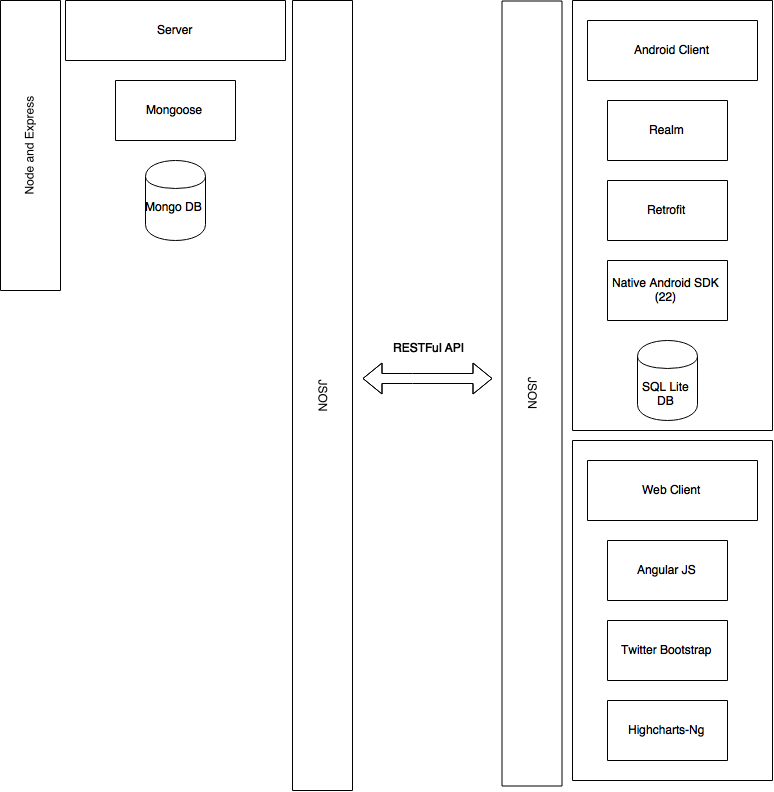
\includegraphics[width=.75\linewidth]{./images/arch.png}} 
  \caption{Proposed Architecture diagram of the system.} 
  \label{fig:Arch}
\end{figure}

The architecture still comprises of the basic 3-tier fundamental framework which follows the Model-View-Controller design pattern. This is present in the web server, web client and android application (adhering to their specific terminology and practices). This complies with the best practices of each of the technologies where given.


\subsection{Web Server}
The web-server is based on a typical client-server communication pattern. The web-based solution is platform independent and mobile responsive.
\subsubsection{Web Server Technology and Design Considerations:} 
The web server utilises a variety of different open source technologies which are all based on Javascript. This allows for the entire web stack to be written in one language.

\textit{Technologies used}
\begin{itemize}
  \item \textbf{MongoDB:} MongoDB is a document based database that utilises a flexible schema \cite{MongoDB}. It is a free and open-source technology.
  \item \textbf{NodeJS:} NodeJS is a Javascript. It uses an event-driven, non-blocking I/O approach that makes it efficient and lightweight \cite{NodeJS}
  \item \textbf{ExpressJS:} Express JS is a minimal web framework for Node JS applications. It provides libraries that allow for the easy development of web solutions using NodeJS \cite{ExpressJS}. The solution api is created using ExpressJS and is represented in Appendix J.
  \item \textbf{Yeoman:} Yeoman allows you to quickly start-up new projects. It prescribes best practices and tools to allow for the development of applications as quickly as possible \cite{Yeoman}. It makes use of open-source generators to scaffold sections of code that would otherwise be repetitive in nature.
  \item \textbf{Angular-Fullstack template from Yeoman:} The angular-fullstack generator is adapted from the angular generator initially created by the yeoman team \cite{AngularFullstack}.
\end{itemize}

\textit{Design Considerations} \\\\
The time-frame of the given project indicated that speed of development needed to be a consideration when building the solution. The \textit{flexible schema} of the Mongo database allows for a schema to be defined in the application code and thus resulted in improved speed of development. Using Mongo in conjunction with Yeoman and the Angular-Fullstack generator, the team leverage off of the advantages offered by these technologies in terms of speed to improve the time of delivery of the solution.\\\\
The generated base framework provided by Yeoman and the Angular-Fullstack makes use of the model-view-controller design pattern on both the client and server. This design pattern allows for the separation of concerns by splitting the logic into the following:
\begin{itemize}
	\item a model that describes the object
	\item the controller that modifies the object, and
	\item the view that handles how the object data will be displayed \cite{MVC}
\end{itemize}
This allowed the team to further build on top of the generated framework using the same best practices and design patterns. The creation of a RESTful API allowed for more extensibility of the solution. The Android solution in section 5.4 was integrated using the RESTful API.

\subsection{Web Client}
%  ANGULAR CAPTURE 
% ALL FUNCTIONALITY OF WEB CLIENT
%  ALSO INCLUDE REPORTING
\subsubsection{Web Client Technology and Design Considerations:}
The web client utilizes a variety of technologies that allow for rapid front-end development and styling. In using Javascript as the common language across the stack, some considerations were made in order to conform to the language usage. Some of the below mentioned technologies come packaged as part of the Angular-Fullstack generator mentioned above.

\textit{Technologies used}
\begin{itemize}
	\item \textbf{AngularJS:} Angular JS allows for the ability to extend the HTML vocabulary. The result is a more readable and expressive front-end that is quick to develop \cite{AngularJS}.
	\item \textbf{Twitter Bootstrap:} This library utilises HTML, Javascript and CSS to enable the developer to build responsive, mobile first web applications. \cite{TwitterBootstrap}.
	\item \textbf{Highcharts-ng:} This library exposes AngularJS directives that wrap some of the functionality provided in the HighchartsJS library. It allows the developer to create expressive reports (for example: bar-charts and pie-charts) \cite{HighchartsNg}.
\end{itemize}

\textit{Design Considerations} \\\\
The online documentation and community knowledge of the above mentioned technologies meant that the learning curve could be mitigated quickly thus improving the speed of solution development. All the technologies mentioned above make use of Javascript as a development language which is also used on the server side. The use of a common language further sped up development of the solution as a whole.\\\\ Highcharts-ng was selected as an appropriate technology for developing the reports due to its compatibility with AngularJS \cite{Highcharts}.

\subsection{Android Client}
\subsubsection{Architecture}
The architecture of the Android native application complies with the style, practices and features of the native Android SDK \cite{AndroidSDK}. The native application of SirVey consists of two activities a "MainActivity" and a "AnswerSurveyActivity". The initial view that the user experiences is designed to be user friendly, touch friendly and responsive. The user is presented with a sliding tab menu composed of a fragments which enable the views to be dynamic provide the user with the best experience possible. 

The main screen consists of a "MainActivity" which comprises of a fragment managing object controlling two fragments a Surveys" fragment and a "Settings" fragment. The "Surveys" fragment is responsible for displaying surveys, displaying the number of completed surveys in local storage and providing navigation to a specific survey which is intended to be answered. The "Settings" fragment is responsible for all use cases pertinent to communicating with the server and device specific operations such as configurations. The "AnswerSurvey" activity is responsible for dynamically producing a form which a surveyor can utilise to answer a survey given a community responses. This activity is pragmatically generated based on the survey data that is provided to it. Thus as new answer types are created in the future such as a "image" answer the only extension is to create a view to represent the new answer type. 

\subsubsection{Technologies used}
The Android application utilises as much of the provided SDK in order to create a dynamic, any screen and user experience which is easy to use and friendly. The local storage also utilises Realm  for local storage which does not use SQLLite but a C++ native hardware storage system that provides faster queries and better performance \cite{RealmPerformance}. Communication utilises RESTful services through Retrofit \cite{retrofit} which enables easily expandable interfaces and complies with web technology.

\subsubsection{Native Application Solution Performance}
The Android application takes advantage of the features of a native development initiative. It is responsive, provides local storage, features the future possibility of incorporating device hardware features (camera, GPS) and allows for easy distribution through an application store. The application provides surveyors with a fast, easy to use and friendly interface in which to capture responses to surveys. It does aid in meeting the success criteria of the platform.

\section{Overall Critical Analysis and Evaluation}

\subsection{Critical Analysis}


\subsubsection{Project Execution}
While critically analysing the project execution phase of the project the team identified some key positives and negatives. These in retrospect should be used as lessons learnt for the next project and guide the team to repeat the positives and learn from the negatives.

\textit{Positives:}

\begin{itemize}
\item The first of which was how the initial POCs were explored: four concurrent POCs were developed in support of “fail fast” strategy \cite{Fail}. This was done so that a failing technology choice could be identified as soon as possible and resources reallocated efficiently.
\item The team utilised collocation to its advantage with regards to requirement specifications and refinements, project progress tracking, acceptance testing, misunderstanding resolution and general team development. 
\item The freedom to attempt any tasks provided self organisation within the team and the collocation assisted in seeing any of the more challenging tasks through.
\item The skills brought into the team by individuals from different working environments were seen as a major positive. These skills and perspectives are leveraged in order to produce the solution provided.
\item The SCRUM methodology chosen is highly collaborative, each team member is able to work independently and share work with other team members by using technologies such as Github \cite{GitHub}. 
\end{itemize}

\textit{Negatives:}

\begin{itemize}
\item The first being that even though opting to go with many POCs provided valuable insight as to which technology would prove successful as early as possible, time was lost that could have been used to focus on one specific technology stack.
\item The team underestimated the amount of effort that would go into the development of the final solution and the time required to introduce 
\end{itemize}

\subsubsection{Project Engineering}

Critical analysis of the project engineering has identified some positives and negatives the team can take advantage of the positives and learn from the negatives for future projects. 

\textit{Positives:}

\begin{itemize}
\item The Android application takes advantages of the benefits of native application development such as performance (user experience and application wise), device hardware and provisioning devices for the users as it is available on a central application store.  
\item The platform provides multiple channels for surveyors to interact with through an Android and web client which leverage on new technology and can be run on hand held devices. 
\item The platform provides surveyors with multi-channel access to the server by either being utilised on a web browser or through a device which can utilise an application store, therefore there is very little set-up or installation required by the surveyors to capture surveys. 
\item The technology stack of the web server and web client uses the same language for all the layers (Javascript) within the stack from the front end to the database.
\end{itemize}

\textit{Negatives:}

\begin{itemize}
\item Due to time constraints on the project the delivery of the project super seeded the requirement to implement industry best practices and standards in certain areas.
\item The API (Application programming interface) has no security and can essentially be called by any browser or web service, security will have to be implemented in a future iteration.
\item Although the software stack allows for excellent automated testing the application lacks significant automated tests mainly due to time constraints with the project. Most of the testing has been done manually.
\item The native android application will require constant maintenance to keep it up to date. As soon as a new version of the android OS is released there is a chance that the APIs or libraries which the application uses can become deprecated. Future sprints will be required to keep the mobile platform up to date. 
\end{itemize}

\subsection{Estimates verses Actual effort}
The total effort of the POC amounted to 1139 hours. This meant the project under estimated by a total of 314 hours and over spent on the budget by R 157 000. The additional time was due to underestimation of the external factors faced by the software team, such as planned leave, other commitments, family emergencies and the under estimation in attaining the required skills on the new technology. New technology was the largest contributor to the additional hours as every team member had to learn the basics of the technology to be able to contribute effectively to the overall solution.

\subsection{Economics and Cost Model}

The last element to the cost model is to look at Commercial Off The Shelf Solutions (COTS) solutions (See exisiting solutions section) \cite{ExpertJudgement}. In this case the business stakeholders should be guided by the software architects as perhaps the cost of starting the POC compared to purchasing a COTS product might not make financial sense. The reason for this is due to the economics of scale, the POC would be a custom application and used only by the business stakeholders. Whereby the COTS products are used by numerous customers globally that have the same basic requirements and therefore share in the total application cost. In this case the research into the existing solutions has confirmed that they meet the expected minimum requirements. This meant the benefit of adopting a COTS for this project would mean that the solution would be available immediately instead of the 825 estimated hours to build the POC. Another benefit would be that the vendors software teams would maintain the application and support the business stakeholders via the support agreements included in the subscription fees. The current assumption based on the actual cost for the SirVey POC is that the business stakeholders would have been able to use the COTS products for +-37 years for the same price the total SirVey POC cost.


\subsubsection{Prototype Licensing}

The prototype is bound by the following licensing agreements.The first being the MIT license (Appendix I) and second being the non-commercial Highcharts JS license. If this application where to be made commercial the Highcharts JS commercial and government license would need to be procured.

\subsection{Evaluation of Output Solution}
% SAY DOES IT MEET SUCCESS CRITERIA .....


\section{Future Work}
The final solution presented in this report is by no means complete and further features could be added to the current prototype. Some of the future features the project team explored where as follows:

\begin{itemize}
\item Add the ability to translate survey and survey questions into other languages. This will allow people to describe a situation they have experienced in their own language and assist the customers in understanding the problems better, thus yielding more accurate survey responses.
\\
\item Incorporate geospatial information into the full application stack. This would leverage the standard GPS units that mobile devices are shipped with. Thus allowing the coordinates to be captured with every survey and used to plot the location. This information can then be plotted onto a map showing the exact location where the survey was captured (see Figure ~\ref{fig:gps}). 

\begin{figure}[H]
	\center{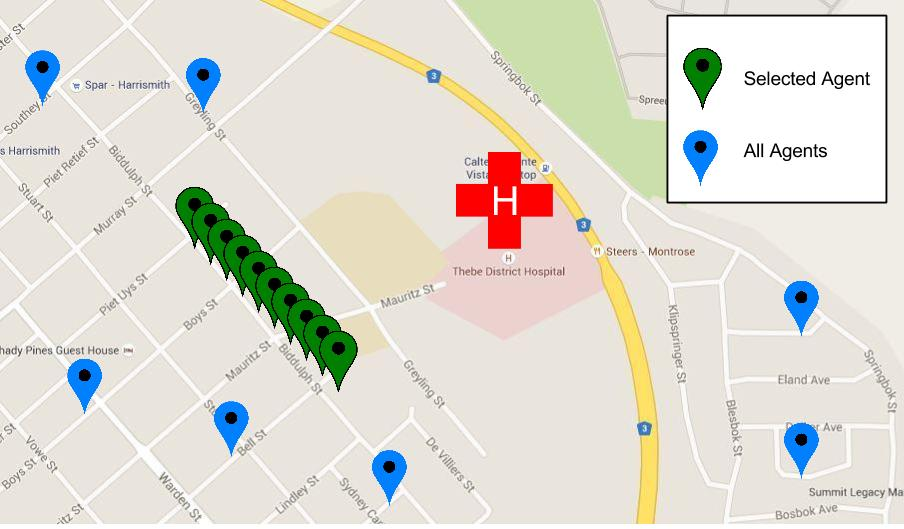
\includegraphics[width=.85\linewidth]{./images/gps}} 
	\caption{GPS coordinates where surveys have been captured.} 
	\label{fig:gps}
\end{figure}

\item Add additional security to the application, currently the integration uses the HTTP protocol which is not secure. The application should be enhanced to use the HTTPS secure protocol. Another security enhancement would be to secure the data stored on the mobile devices as well as the master database. Thus could be achieved by encrypting with 128 Bit Advanced Encryption Standard (AES) \cite{AES}. \\ \\

\item The prototype was build exclusively for the Android operating system. As the final enhancement, the application could be extended to other mobile platforms such as Apple's OS X and windows mobile.
\end{itemize}

With the prototype source code freely available within the repository further software teams could collaborate and build the additional features.

%%%%%%%%%%%%%%%%%%%%%%%%%%%%%%%%%%%%%%%%%%%%%%%%%%%%%%%%%%%%%%%%%%%%%%%%%%%%%%%
%
\section{Conclusion}

- team organisation
- methodology
- design considerations
- trade-offs
- critical analysis

%A conclusion may review the main points of the paper, but do not replicate the abstract as the conclusion.



%%%%%%%%%%%%%%%%%%%%%%%%%%%%%%%%%%%%%%%%%%%%%%%%%%%%%%%%%%%%%%%%%%%%%%%%%%%%%%%
%

\newpage
\newcommand{\summary}[1]{\addtocontents{toc}{#1\par}}
\phantomsection
\addcontentsline{toc}{section}{REFERENCES}


\renewcommand{\bibname}{REFERENCES}
\renewcommand*{\bibfont}{\raggedright}

\bibliographystyle{witseie}
\bibliography{references}

\newpage
% %%%%%%%%%%%%%%%%%%%%%%%%%%%%%%%%%%%%%%%%%%%%%%%%%%%%%%%%%%%%%%%%%%%%%%%%%%%%%%%



% \pagestyle{plain}
% \pagenumbering{Alph}
% \renewcommand\thesection{\Alph{section}}
% \setcounter{section}{0}

\section{Appendix A: Requirements Engineering Documentation}

\subsection{Key Examples}

\textbf{Key Examples: Conducting a Survey}
\begin{itemize}
\item Surveyor asks a yes/no question 
\item Surveyor ask a question with pre-defined answers
\item Surveyor asks a free form question
\end{itemize}

\textbf{Key Examples: Reporting}
\begin{itemize}
\item The number of yes/no answers are tallied and displayed per question
\item The number of each pre-defined answer are tallied and displayed per question
\item The number of key phrases are tallied and displayed per free-form answer
\end{itemize}

\textbf{Key Examples: Offline Mode}
\begin{itemize}
\item The surveyor conducts a single survey in offline mode and syncs with the system
\item The surveyor conducts multiple surveys in offline mode and syncs all of them with the system
\end{itemize}

\textbf{Key Examples: Survey Administration}
\begin{itemize}
\item The administrator adds a new survey
\item The administrator edits an existing survey
\item The administrator removes an existing survey
\end{itemize}

\textbf{Key Examples: User Access}
\begin{itemize}
\item A new user of the system registers
\item An existing user logs into the system as an administrator
\item An existing user logs into the system as a non-administrator
\item An existing user changes password
\end{itemize}


\subsection{Specification with Examples}

\textbf{Conducting a Survey}\\
Given that a yes/no question has been defined \\
when the surveyor asks the respondent the question\\
then the surveyor can only capture an answer from the given options\\

Given that a pre-defined question has been defined\\
when the surveyor asks the respondent the question\\
then the surveyor can only capture an answer from the given options\\

Given that a free-form question has been defined\\
when the surveyor as the respondent the question\\
then the surveyor can capture a text answer, limited to 1500 characters\\

\textbf{Reporting}\\
Given that the user is logged in as an administrator\\
then the user has access to the reporting functionality\\

Given that the user is logged in as an administrator\\
and a survey has been conducted\\
and the survey has been submitted\\
and the survey contains yes/no questions\\
or the survey contains pre-defined answers\\
when the survey’s results are selected\\
then a graph showing the responses received is displayed\\

\textbf{Offline Mode}\\
Given the system has no access to the internet \\
and the surveyor has submitted a completed survey \\
then the system should show how many offline surveys have been completed\\

Given that the system has no access to the internet\\
and the system has stored surveys \\
when the administrator syncs the system\\
and there is an internet connection \\
then the surveys get submitted with server\\

\textbf{Survey Administration}\\
Given that a user is logged in as an administrator\\
then the user has access to the create survey functionality\\
and the user has access to the edit survey functionality\\
and the user has access to the delete survey functionality\\

\textbf{User Access}\\
Given that a user has not been registered on the system\\
then the user can register on the system\\

Given that the user has registered on the system\\
then the user can log into the system using their username and password\\
and the user can change their password\\

\newpage
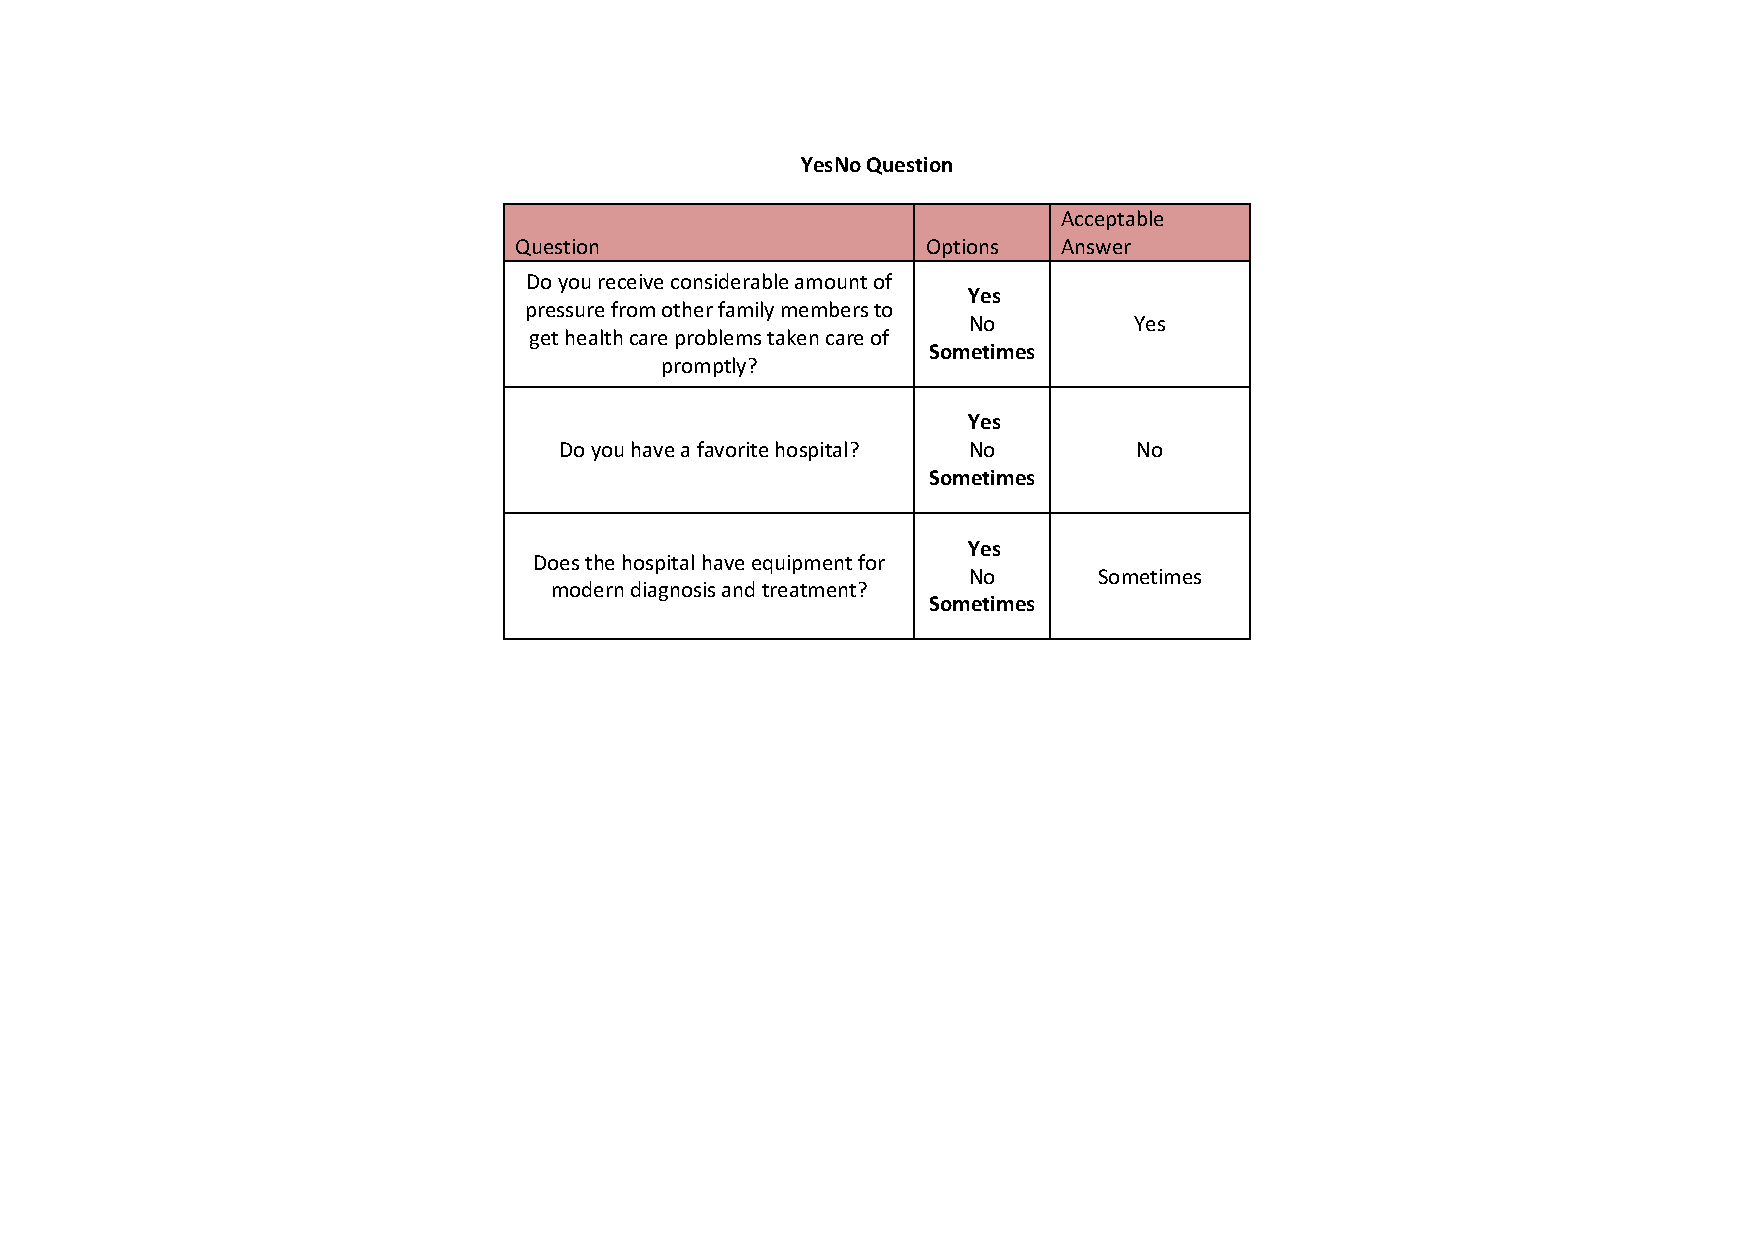
\includepdf[pages=-,pagecommand={\pagestyle{fancy}}]{./Specs/1.pdf}

\begin{figure}[H]
	\center{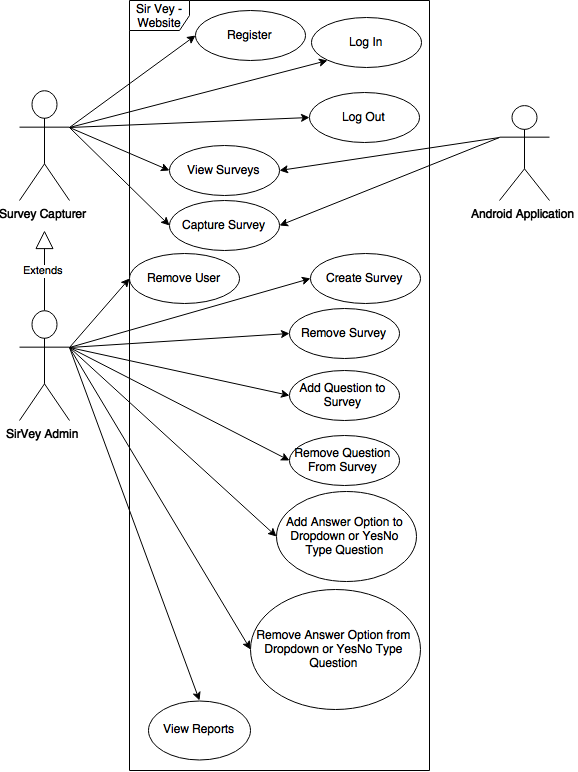
\includegraphics[width=.95\linewidth]{./images/SirVeyUMLDiagram.png}} 
	\caption{Use Case Diagram for SirVey Application.} 
	\label{fig:UseCase}
\end{figure}

\newpage
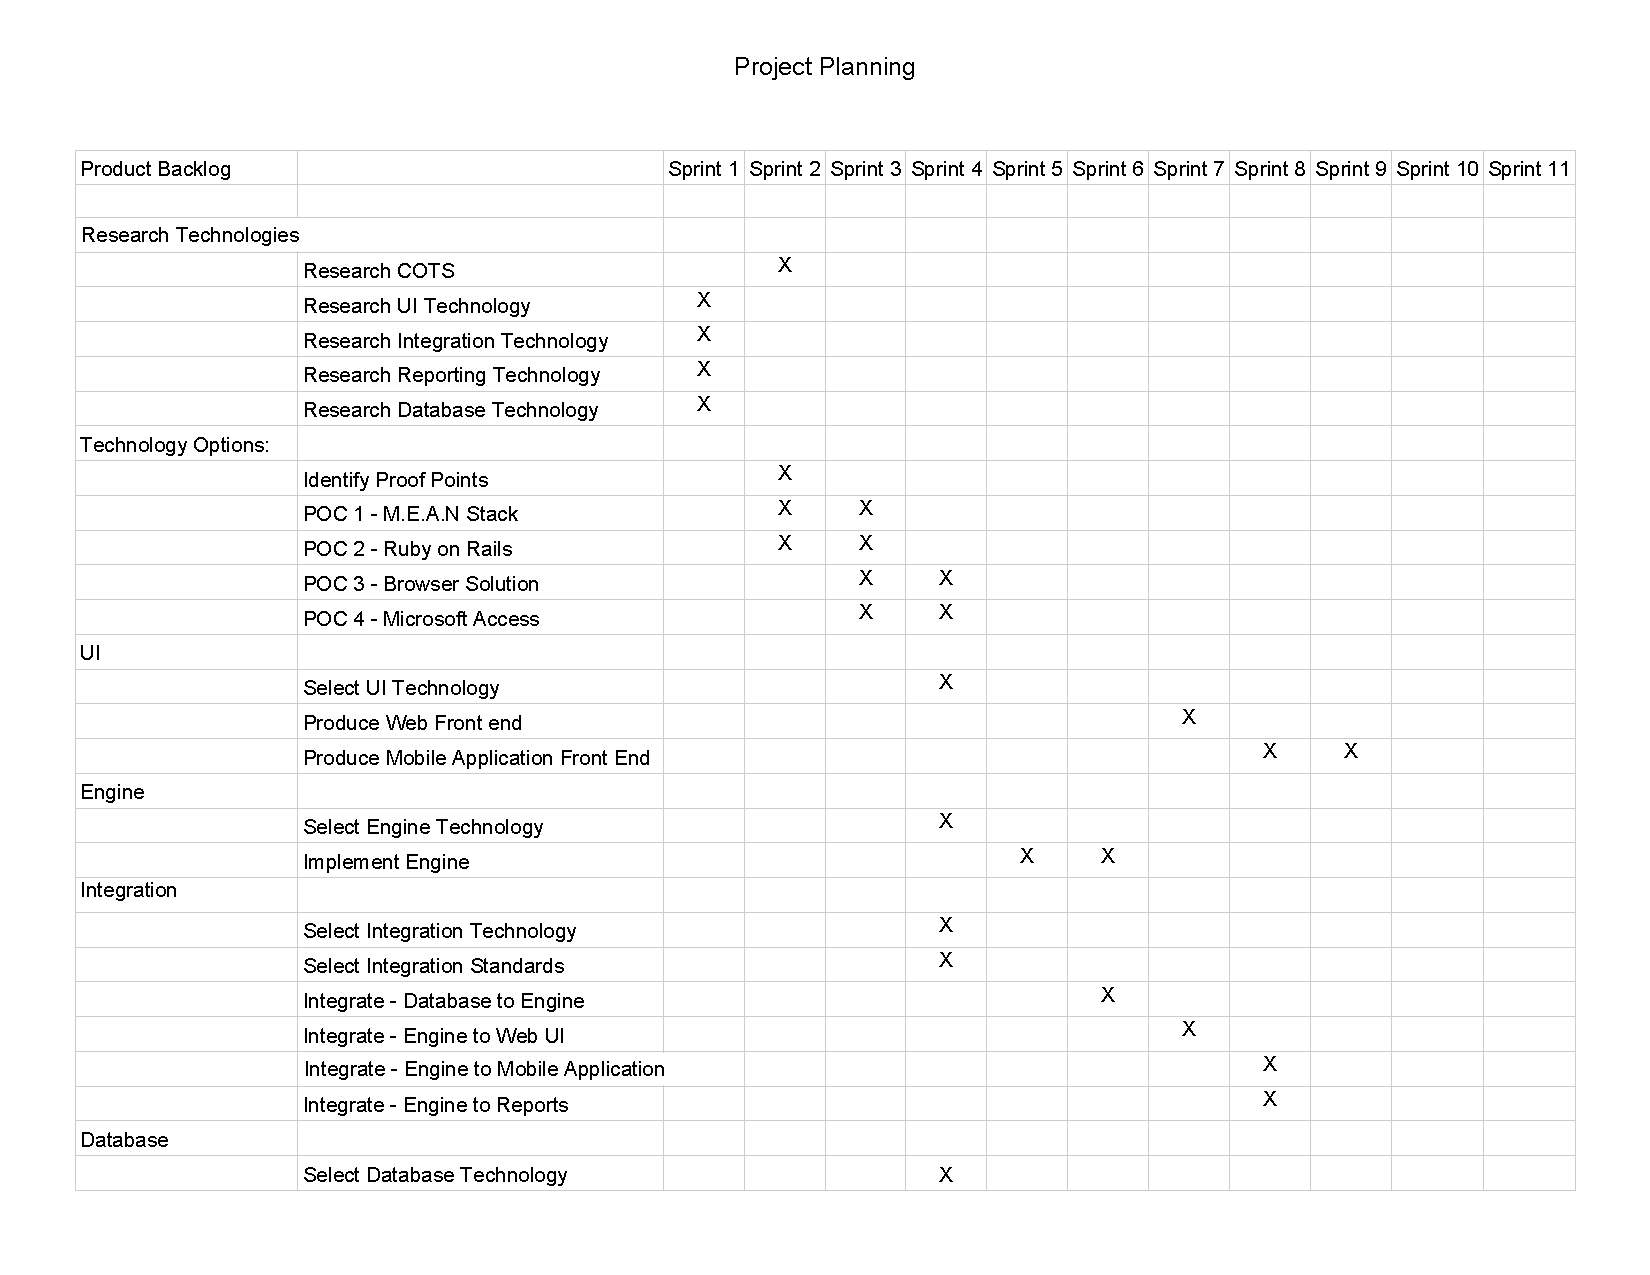
\includepdf[pages=1,pagecommand=\section{Appendix C: Sprint Planning}]{./sprint_planning/ProjectPlanning.pdf}
\includepdf[pages=2-,pagecommand={\pagestyle{fancy}}]{./sprint_planning/ProjectPlanning.pdf}

\newpage
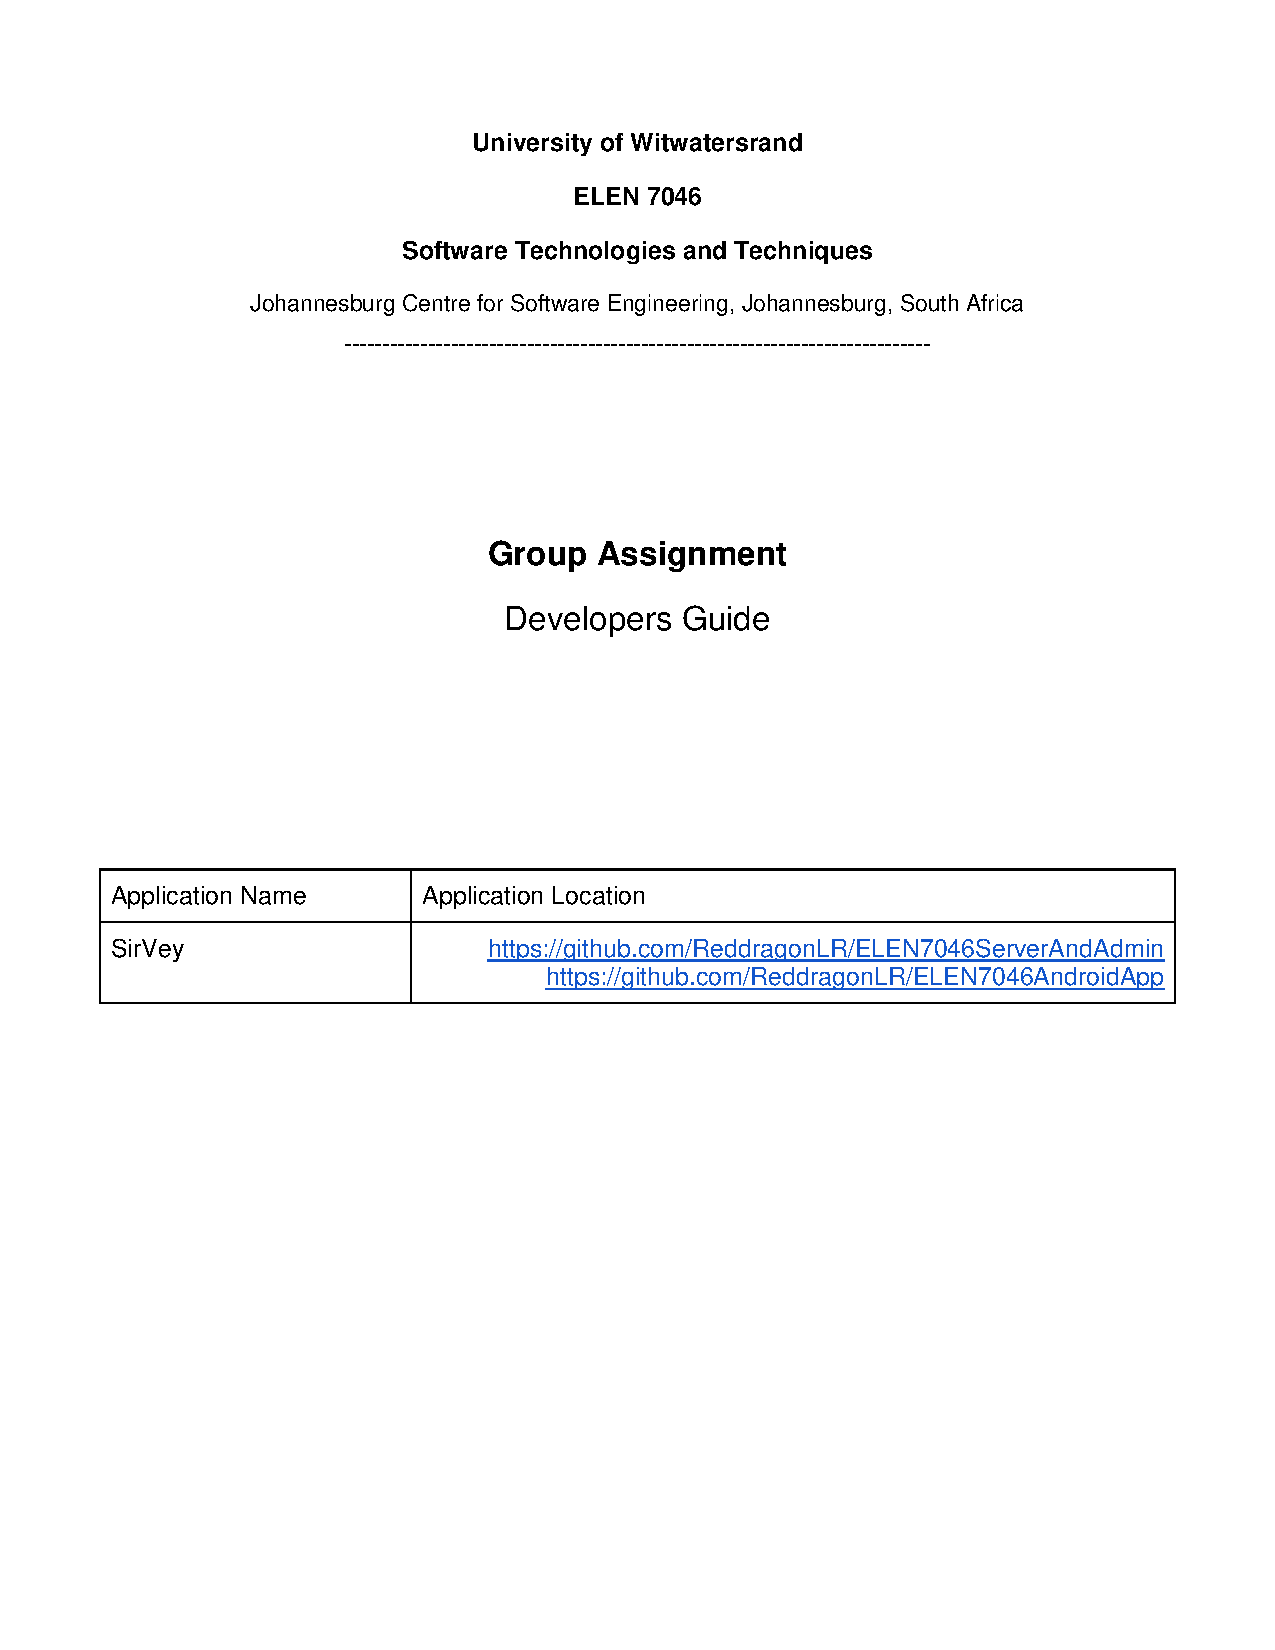
\includepdf[pages=1,pagecommand=\section{Appendix D: Developer Guide}]{./Guides/DevelopersGuide.pdf}
\includepdf[pages=2-,pagecommand={\pagestyle{fancy}}]{./Guides/DevelopersGuide.pdf}

\newpage
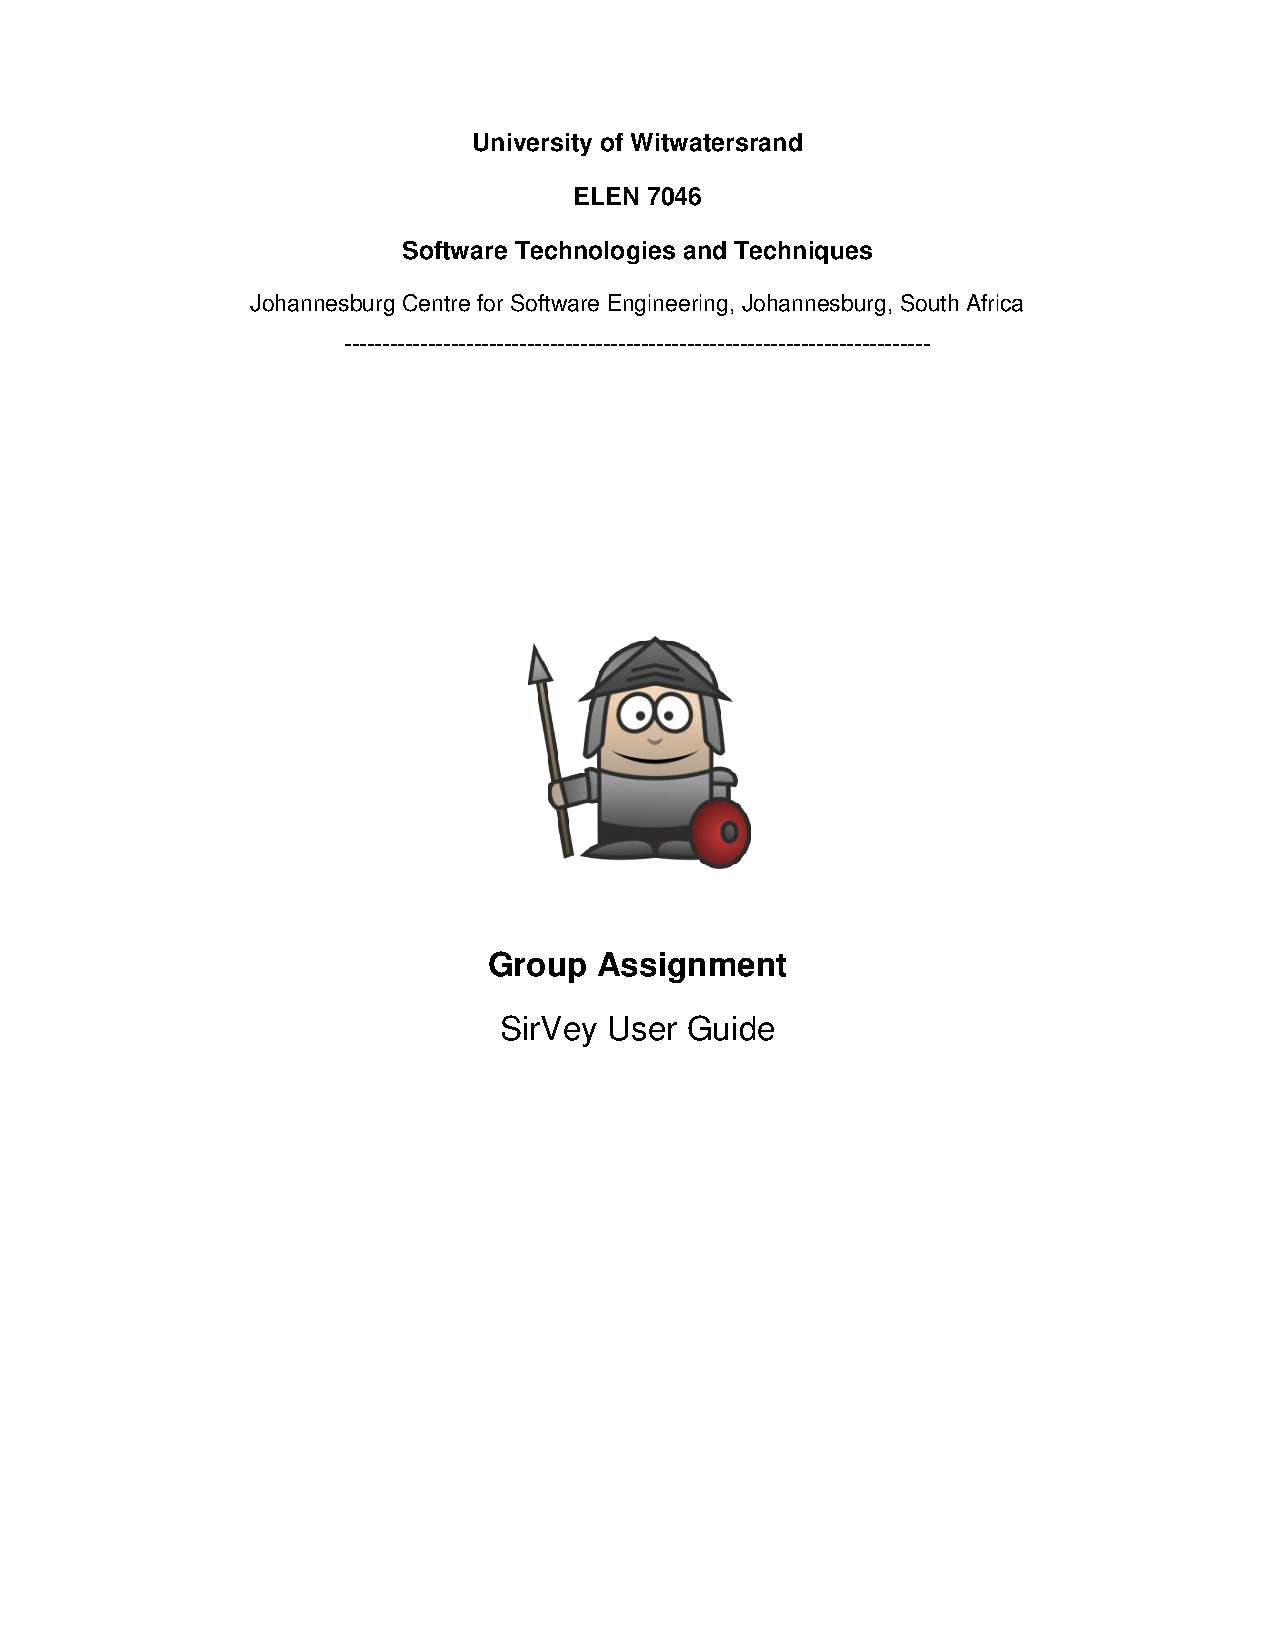
\includepdf[pages=1,pagecommand=\section{Appendix E: User Training Guide}]{./Guides/UserGuide.pdf}
\includepdf[pages=2-,pagecommand={\pagestyle{fancy}}]{./Guides/UserGuide.pdf}

\newpage
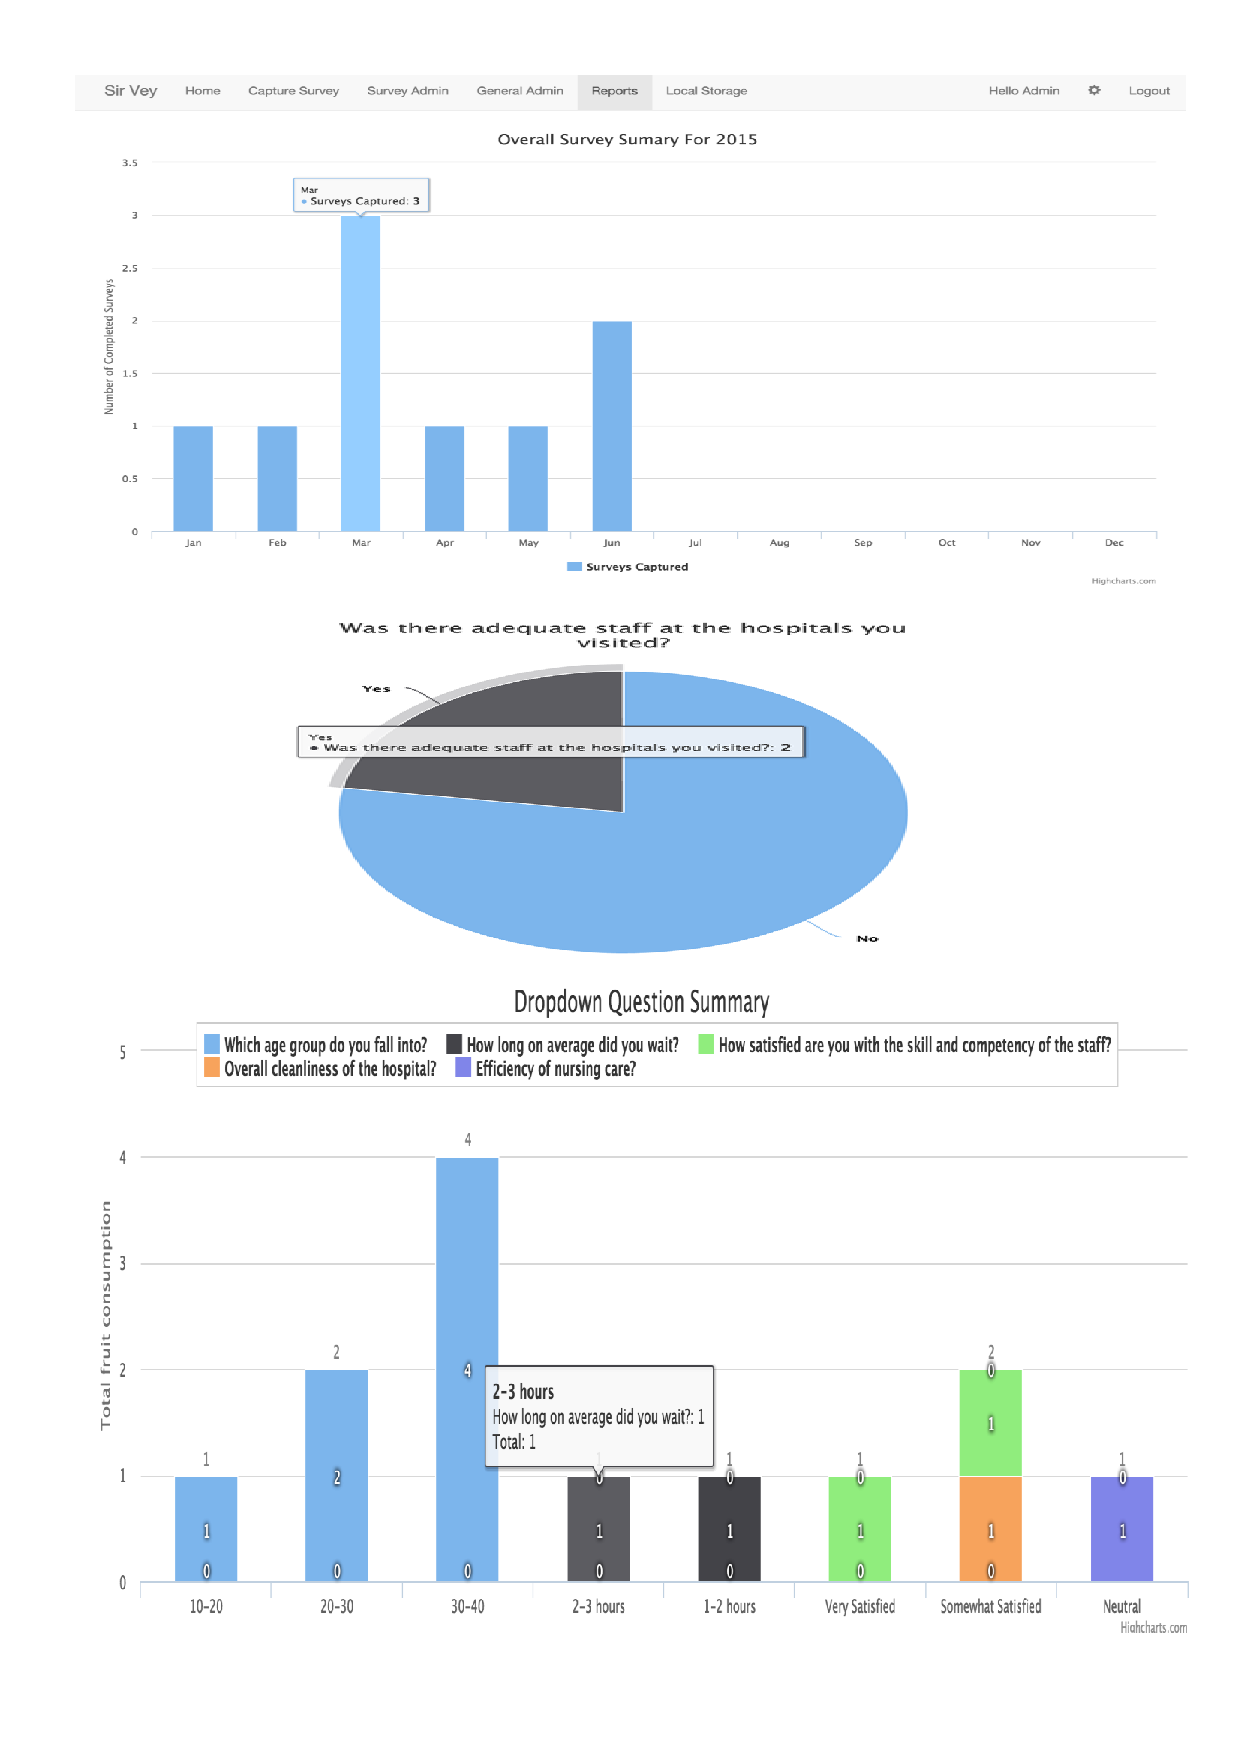
\includepdf[pages=-,scale=0.85,pagecommand=\section{Appendix F: Final prototype Reports}]{./Guides/FinalReports.pdf}

\newpage
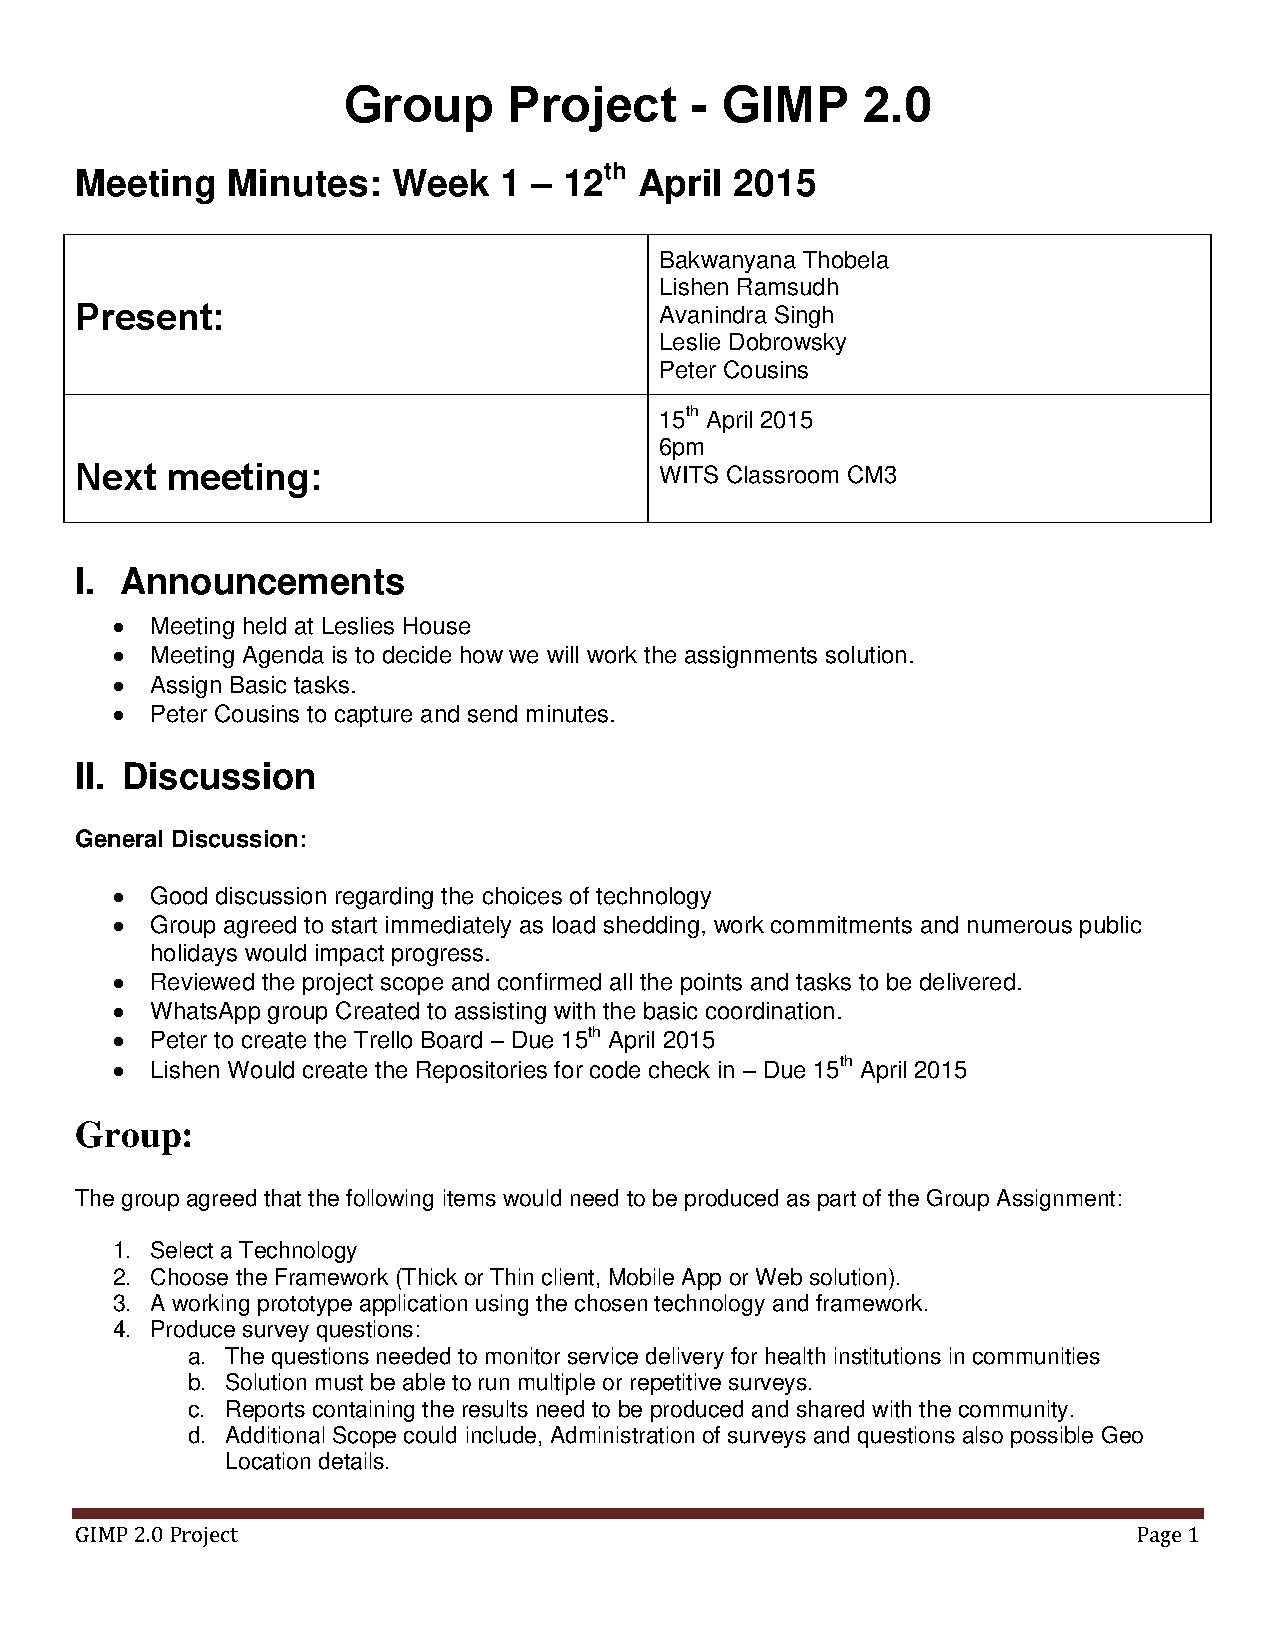
\includepdf[pages=1,scale=0.85,pagecommand=\section{Appendix G: Stand-up Meeting minutes}]{./sprint_planning/1Meeting.pdf}
\includepdf[pages=2-,scale=0.85,pagecommand={\pagestyle{fancy}}]{./sprint_planning/1Meeting.pdf}
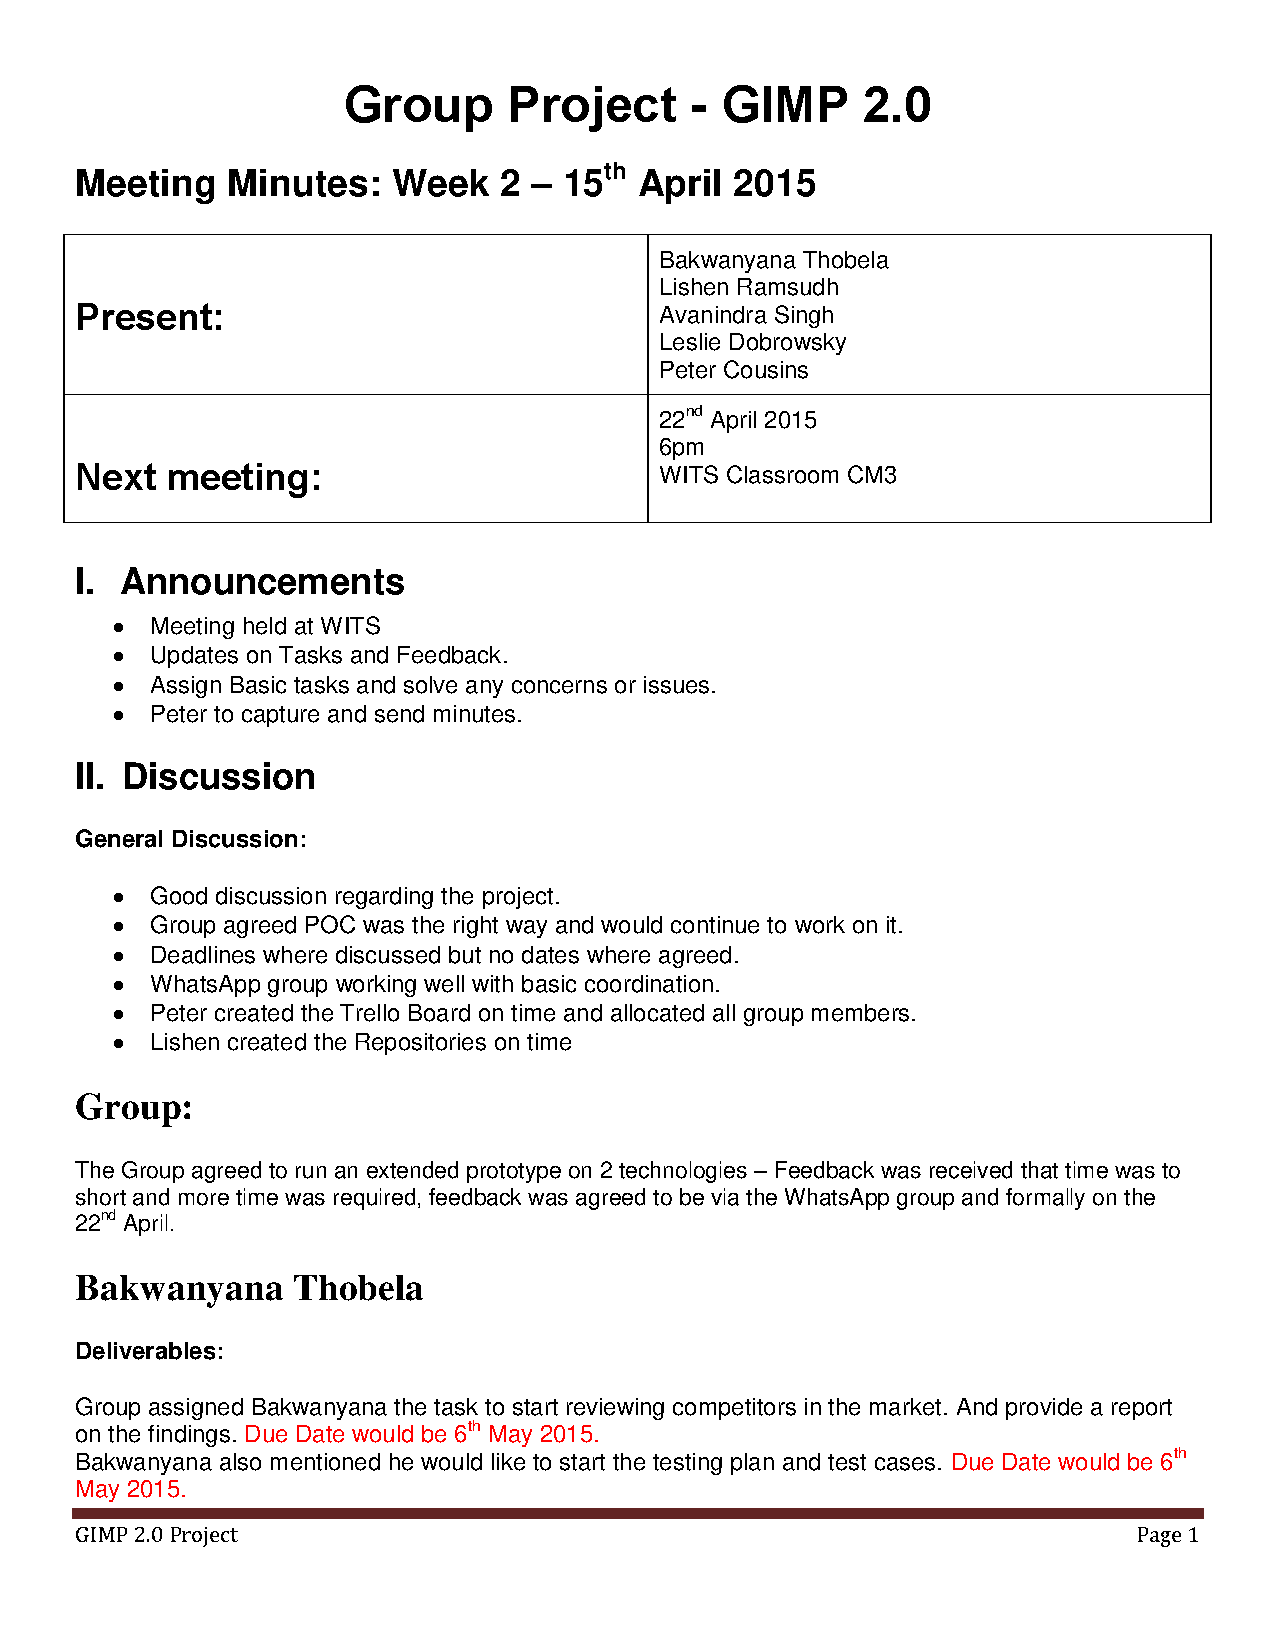
\includepdf[pages=-,scale=0.85,pagecommand={\pagestyle{fancy}}]{./sprint_planning/2Meeting.pdf}
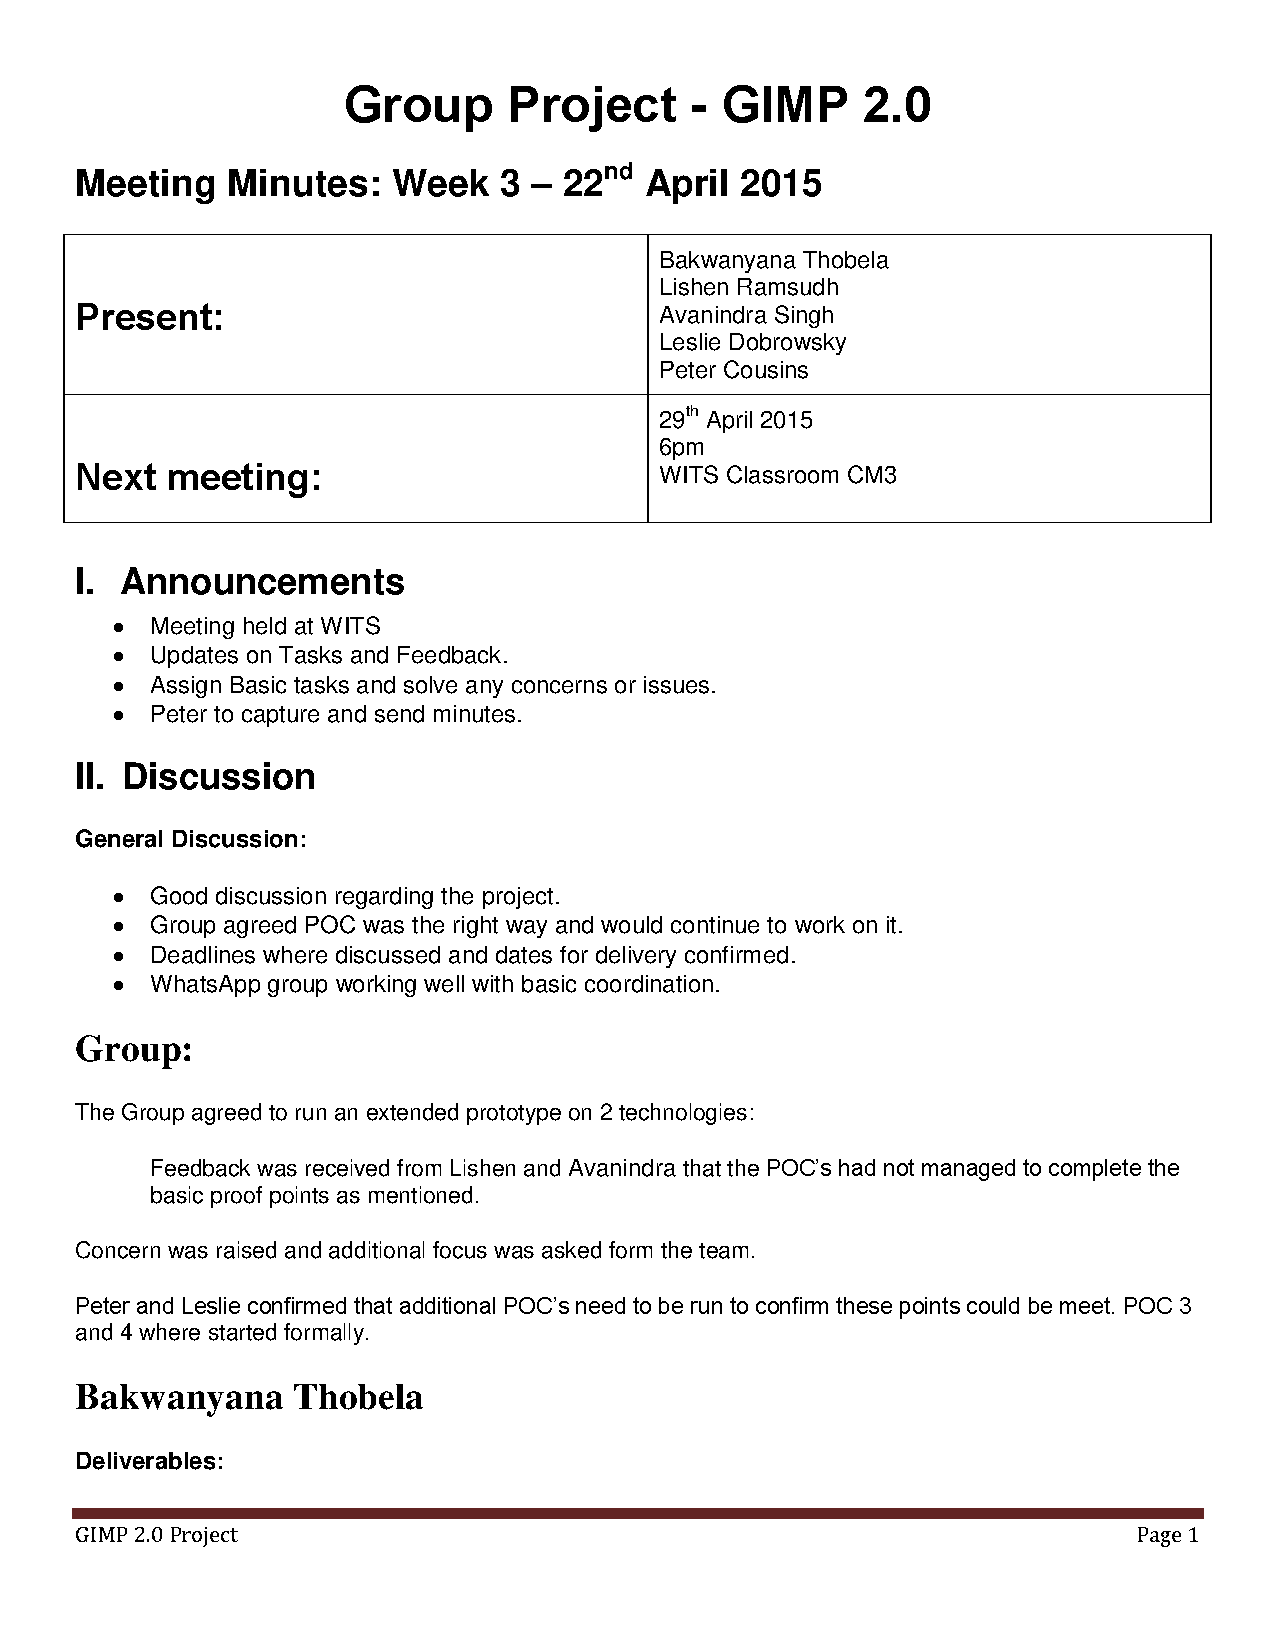
\includepdf[pages=-,scale=0.85,pagecommand={\pagestyle{fancy}}]{./sprint_planning/3Meeting.pdf}
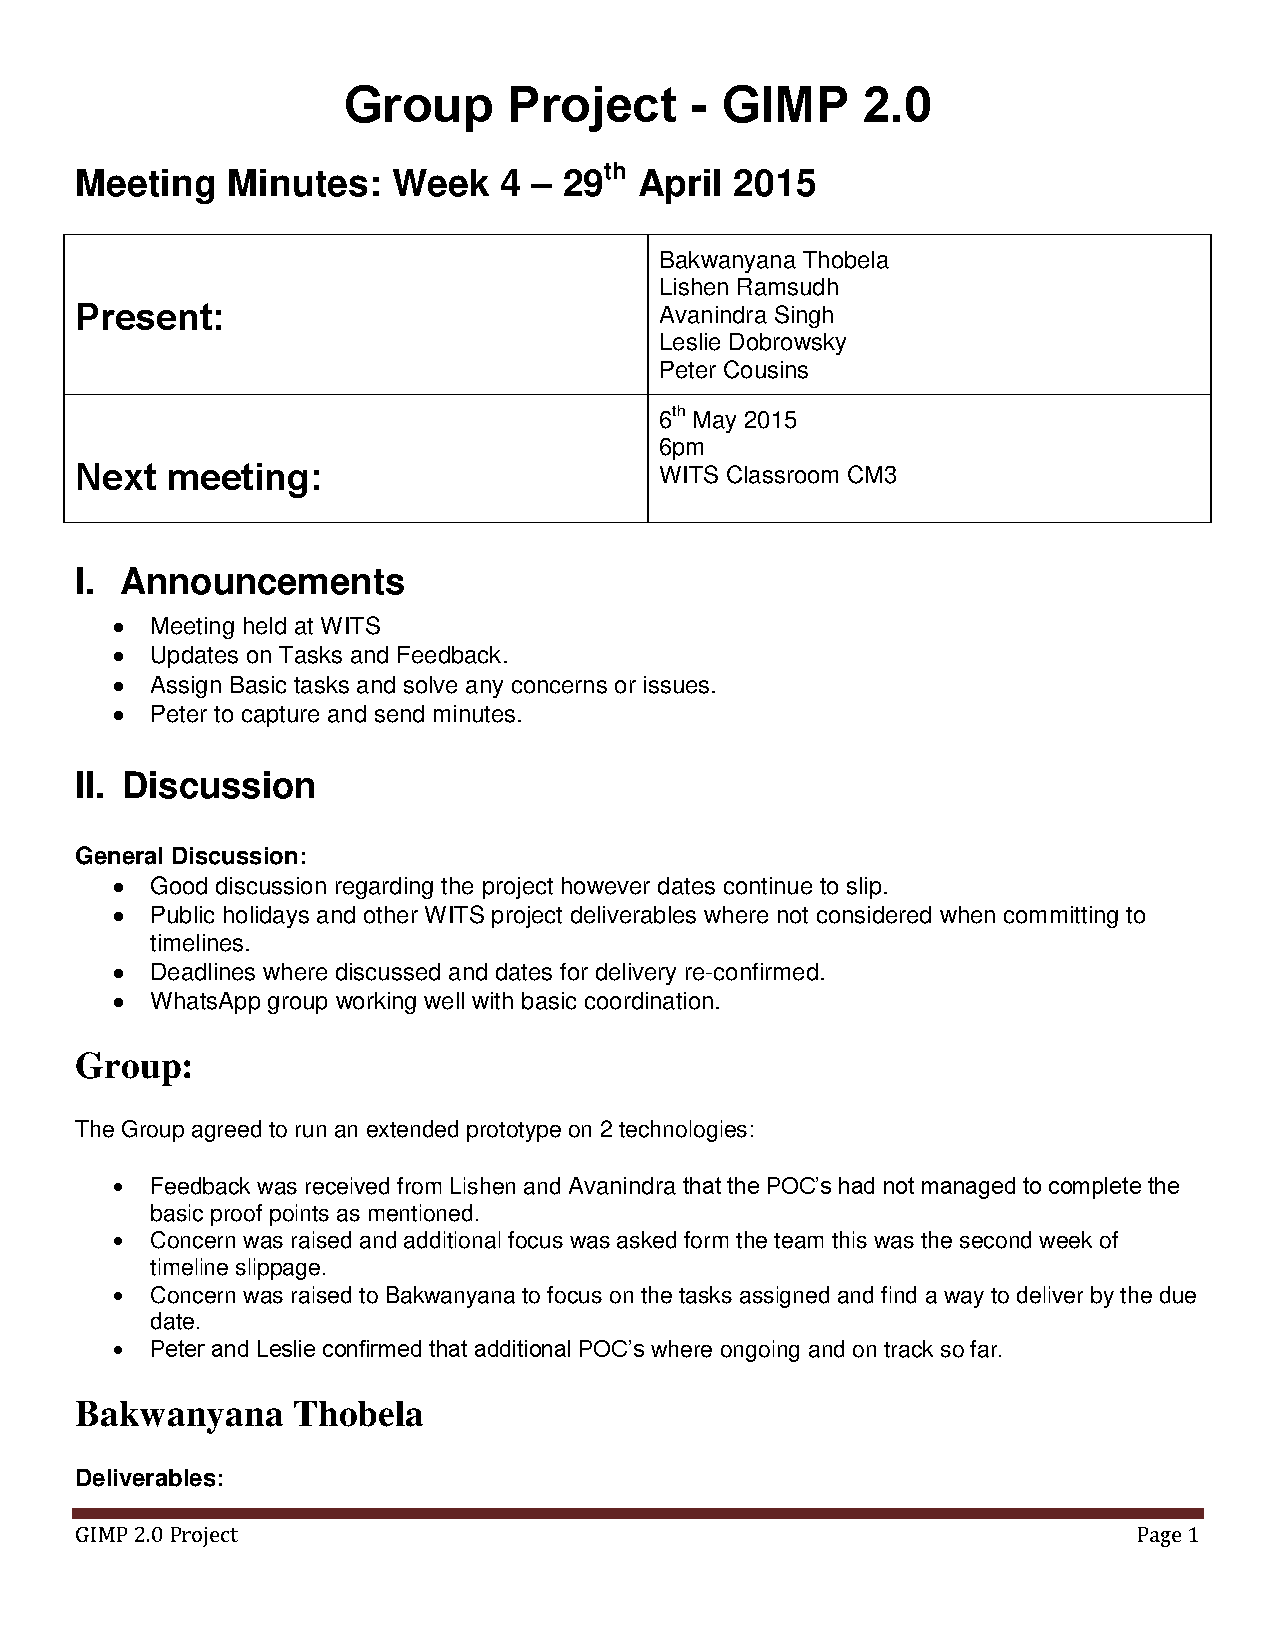
\includepdf[pages=-,scale=0.85,pagecommand={\pagestyle{fancy}}]{./sprint_planning/4Meeting.pdf}
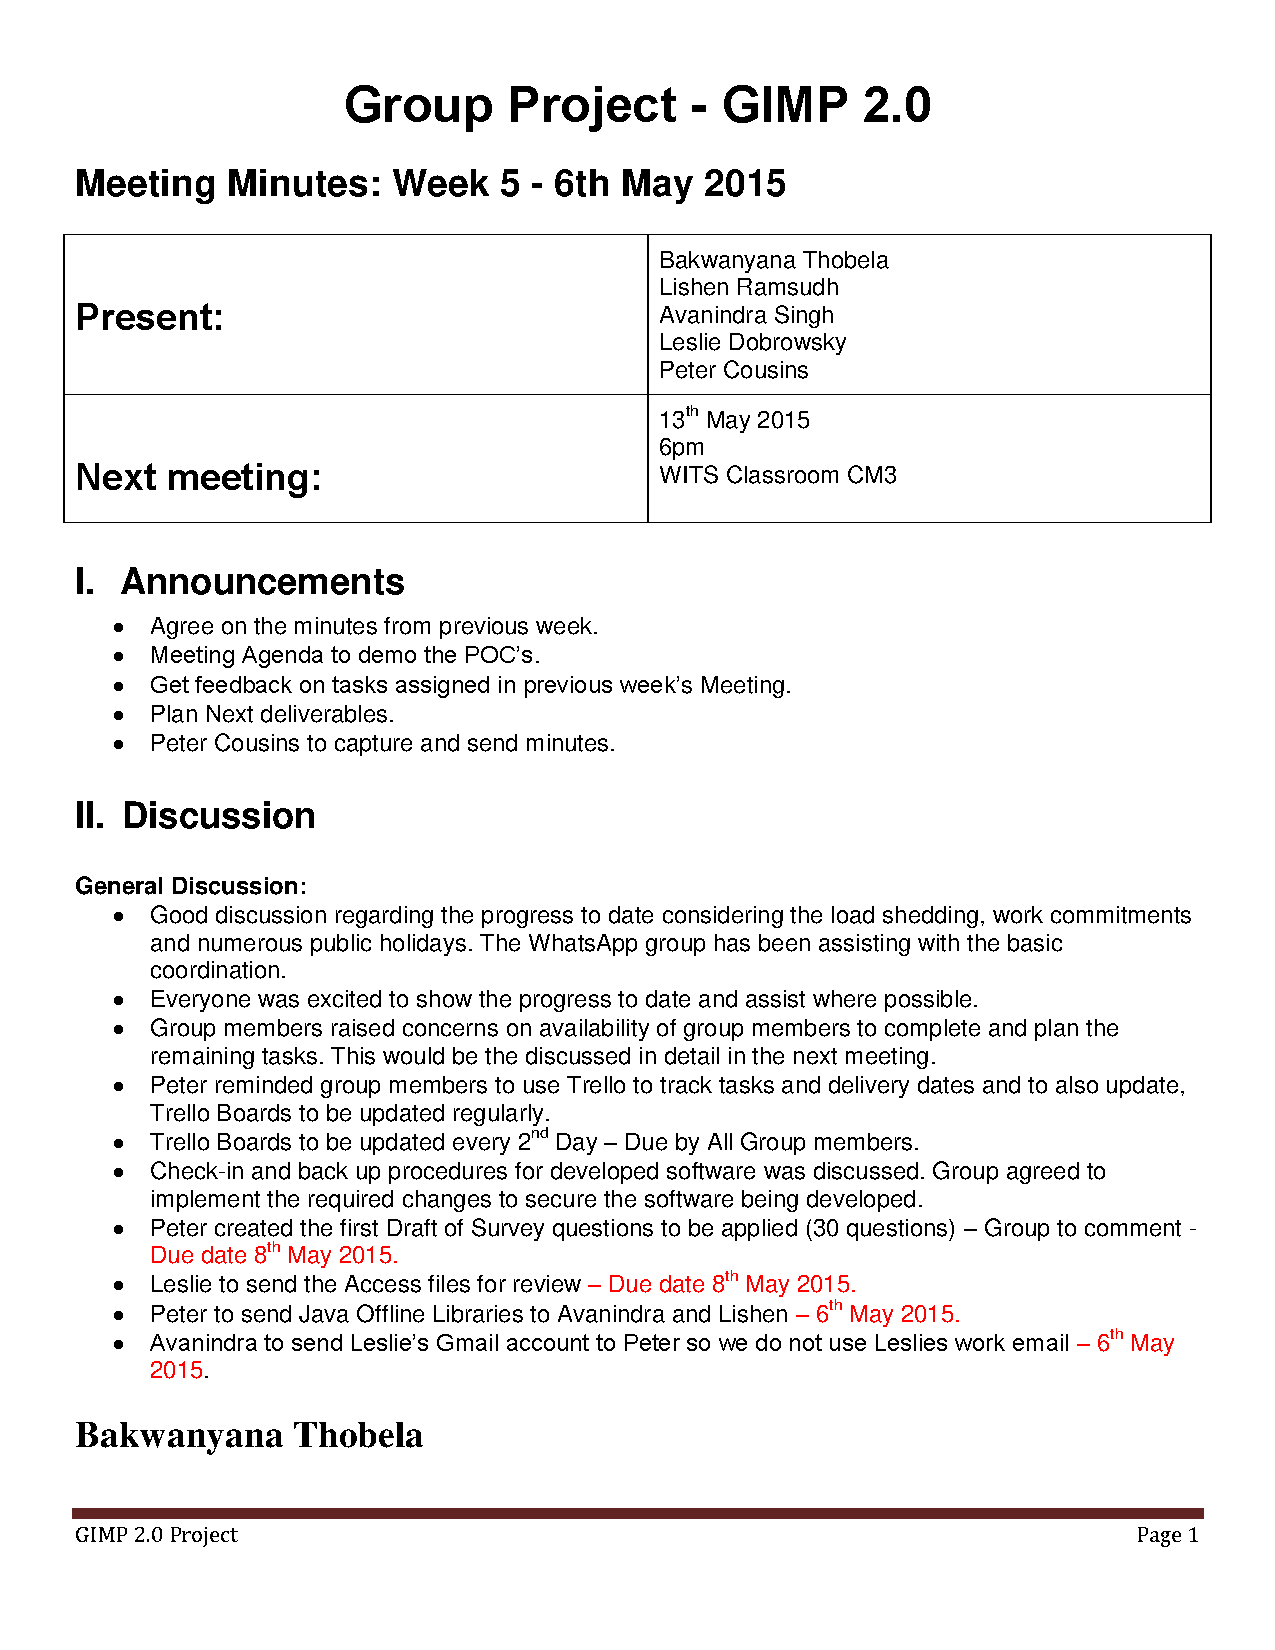
\includepdf[pages=-,scale=0.85,pagecommand={\pagestyle{fancy}}]{./sprint_planning/5Meeting.pdf}
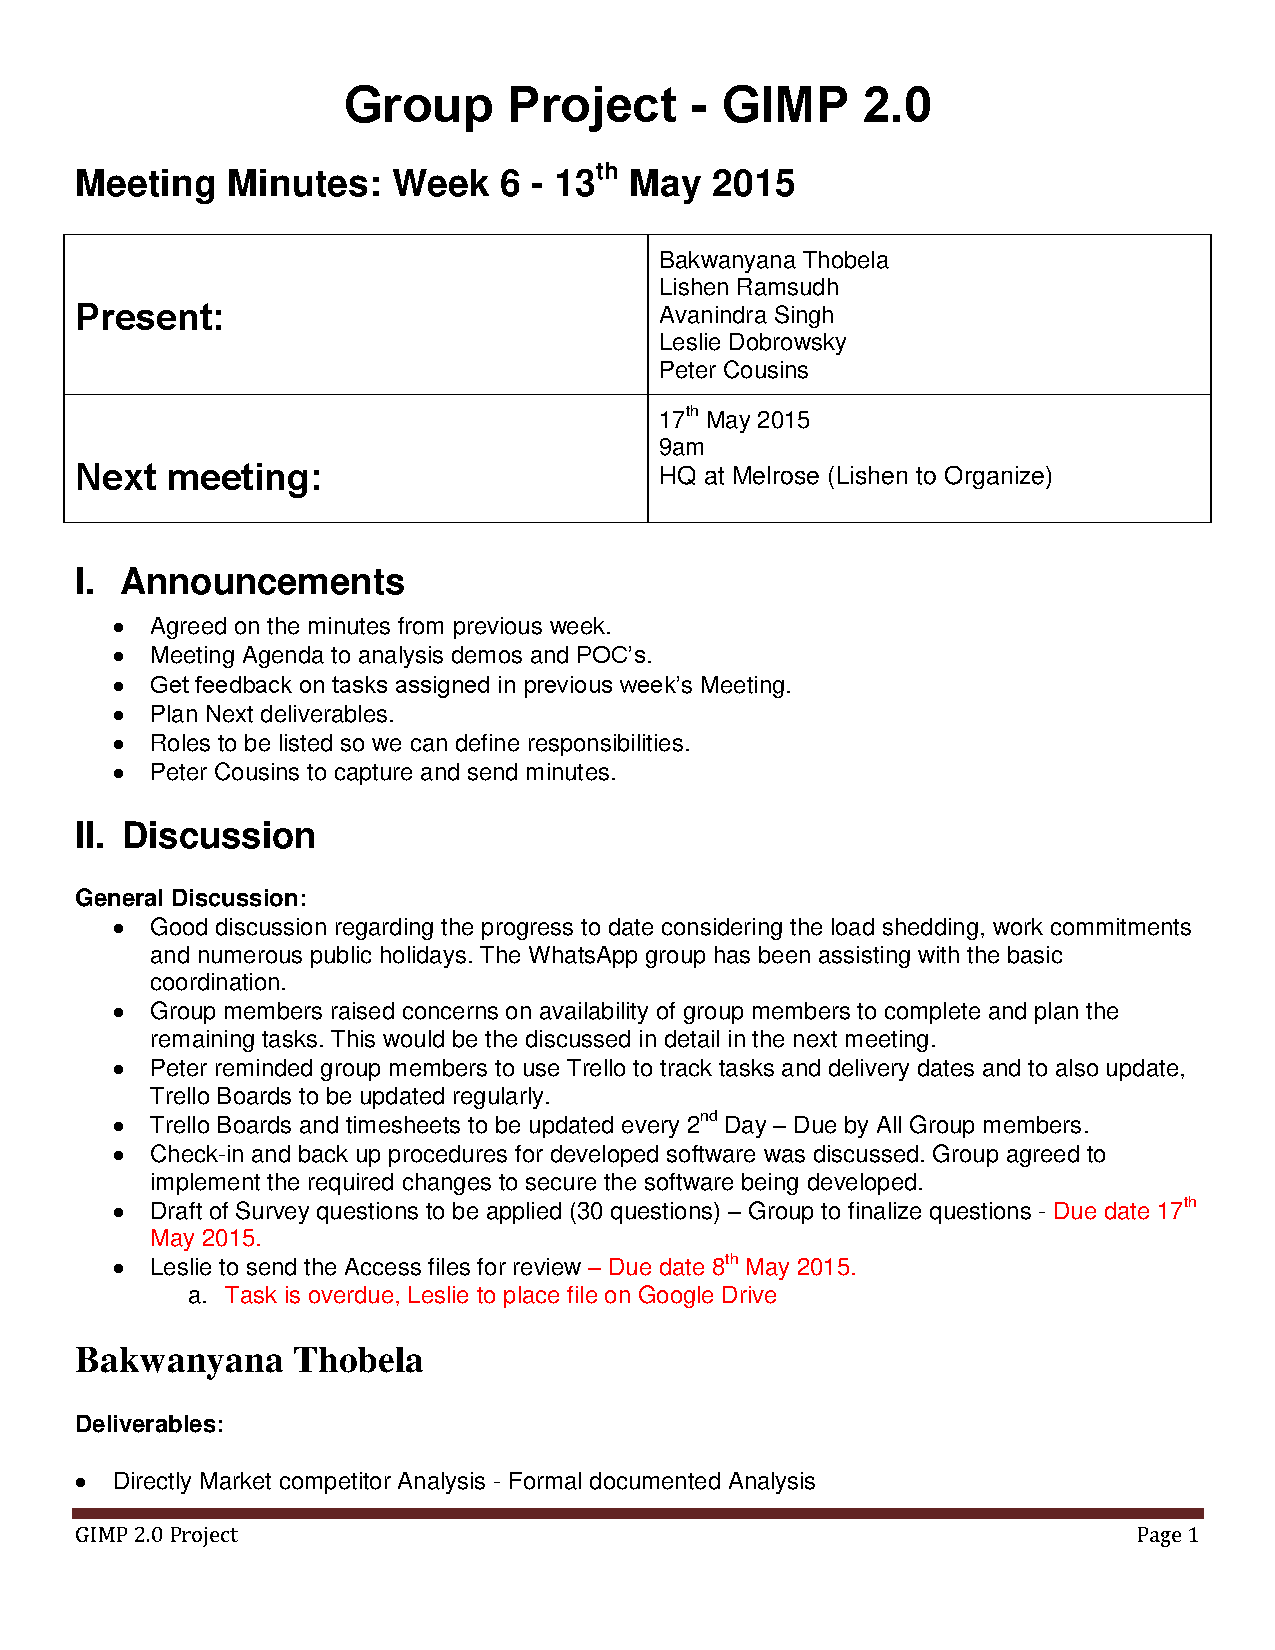
\includepdf[pages=-,scale=0.85,pagecommand={\pagestyle{fancy}}]{./sprint_planning/6Meeting.pdf}
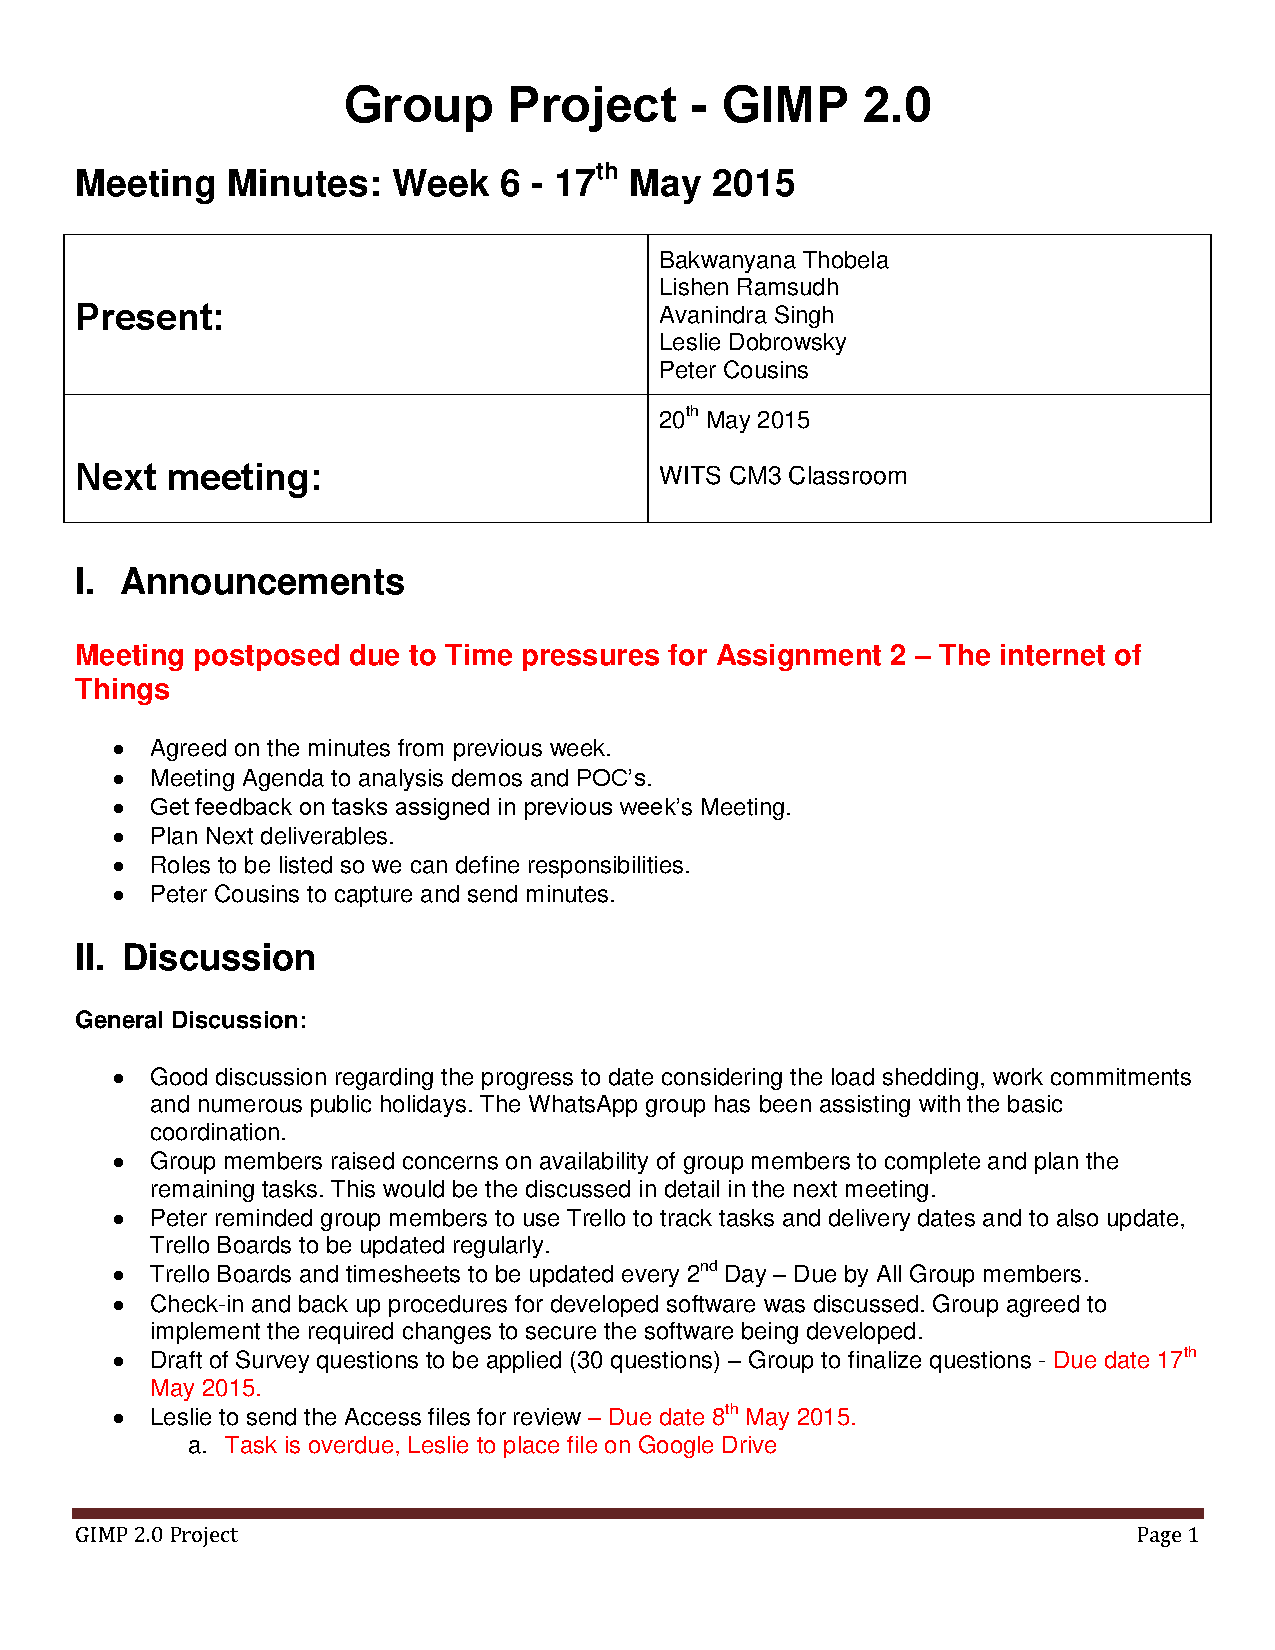
\includepdf[pages=-,scale=0.85,pagecommand={\pagestyle{fancy}}]{./sprint_planning/7Meeting.pdf}
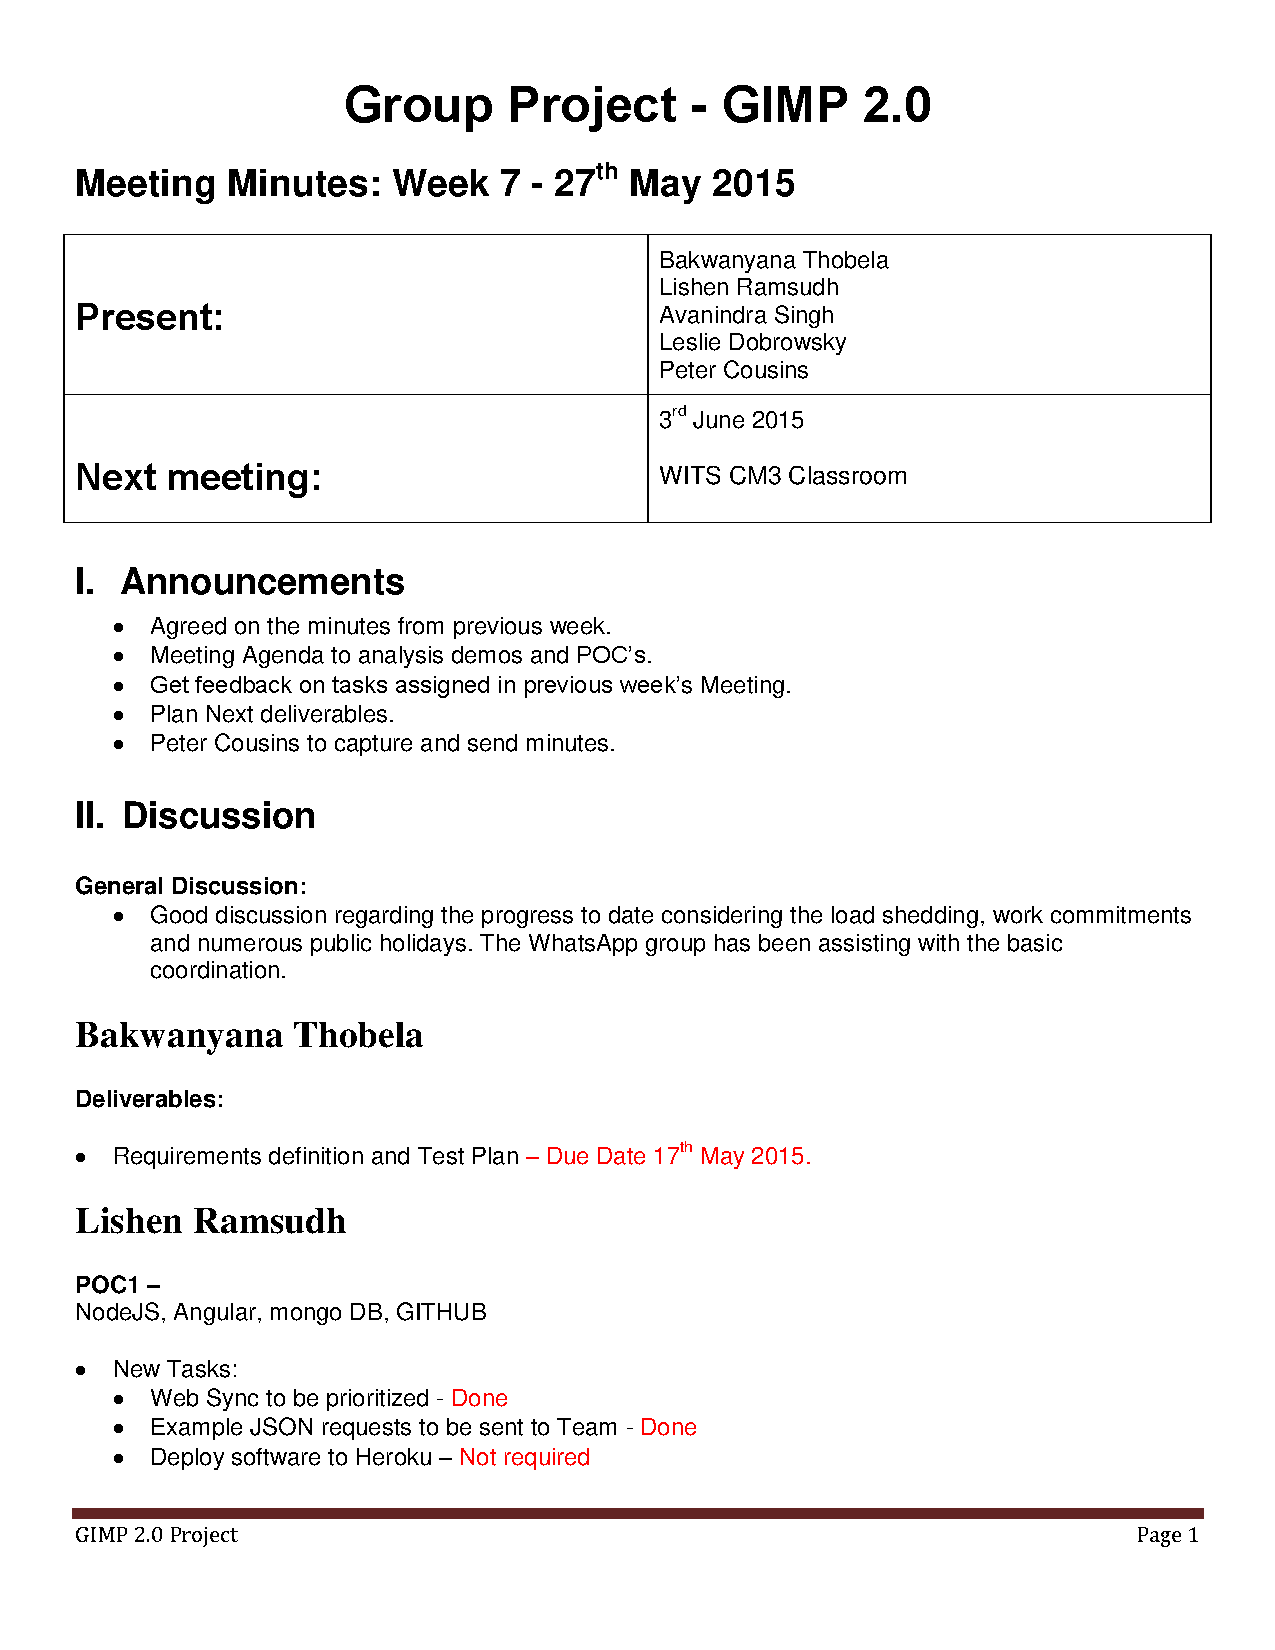
\includepdf[pages=-,scale=0.85,pagecommand={\pagestyle{fancy}}]{./sprint_planning/8Meeting.pdf}
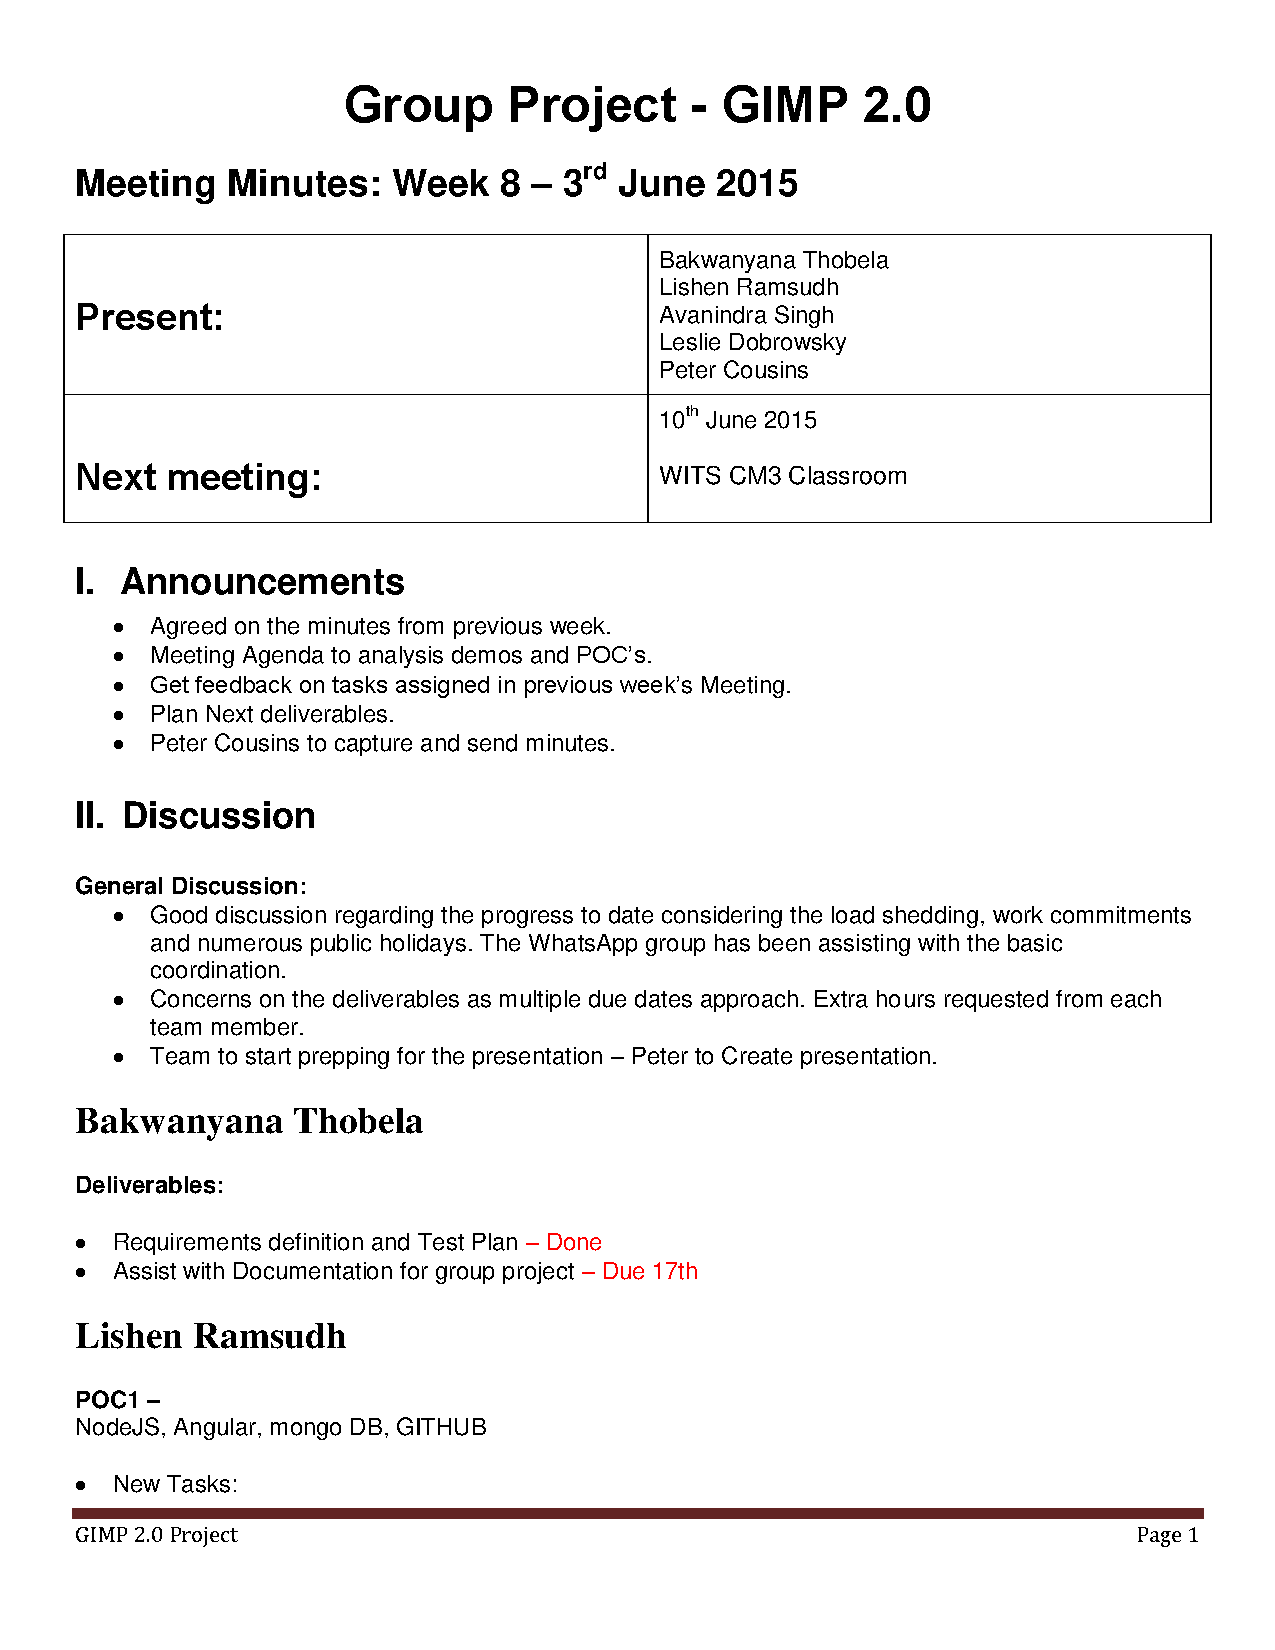
\includepdf[pages=-,scale=0.85,pagecommand={\pagestyle{fancy}}]{./sprint_planning/9Meeting.pdf}
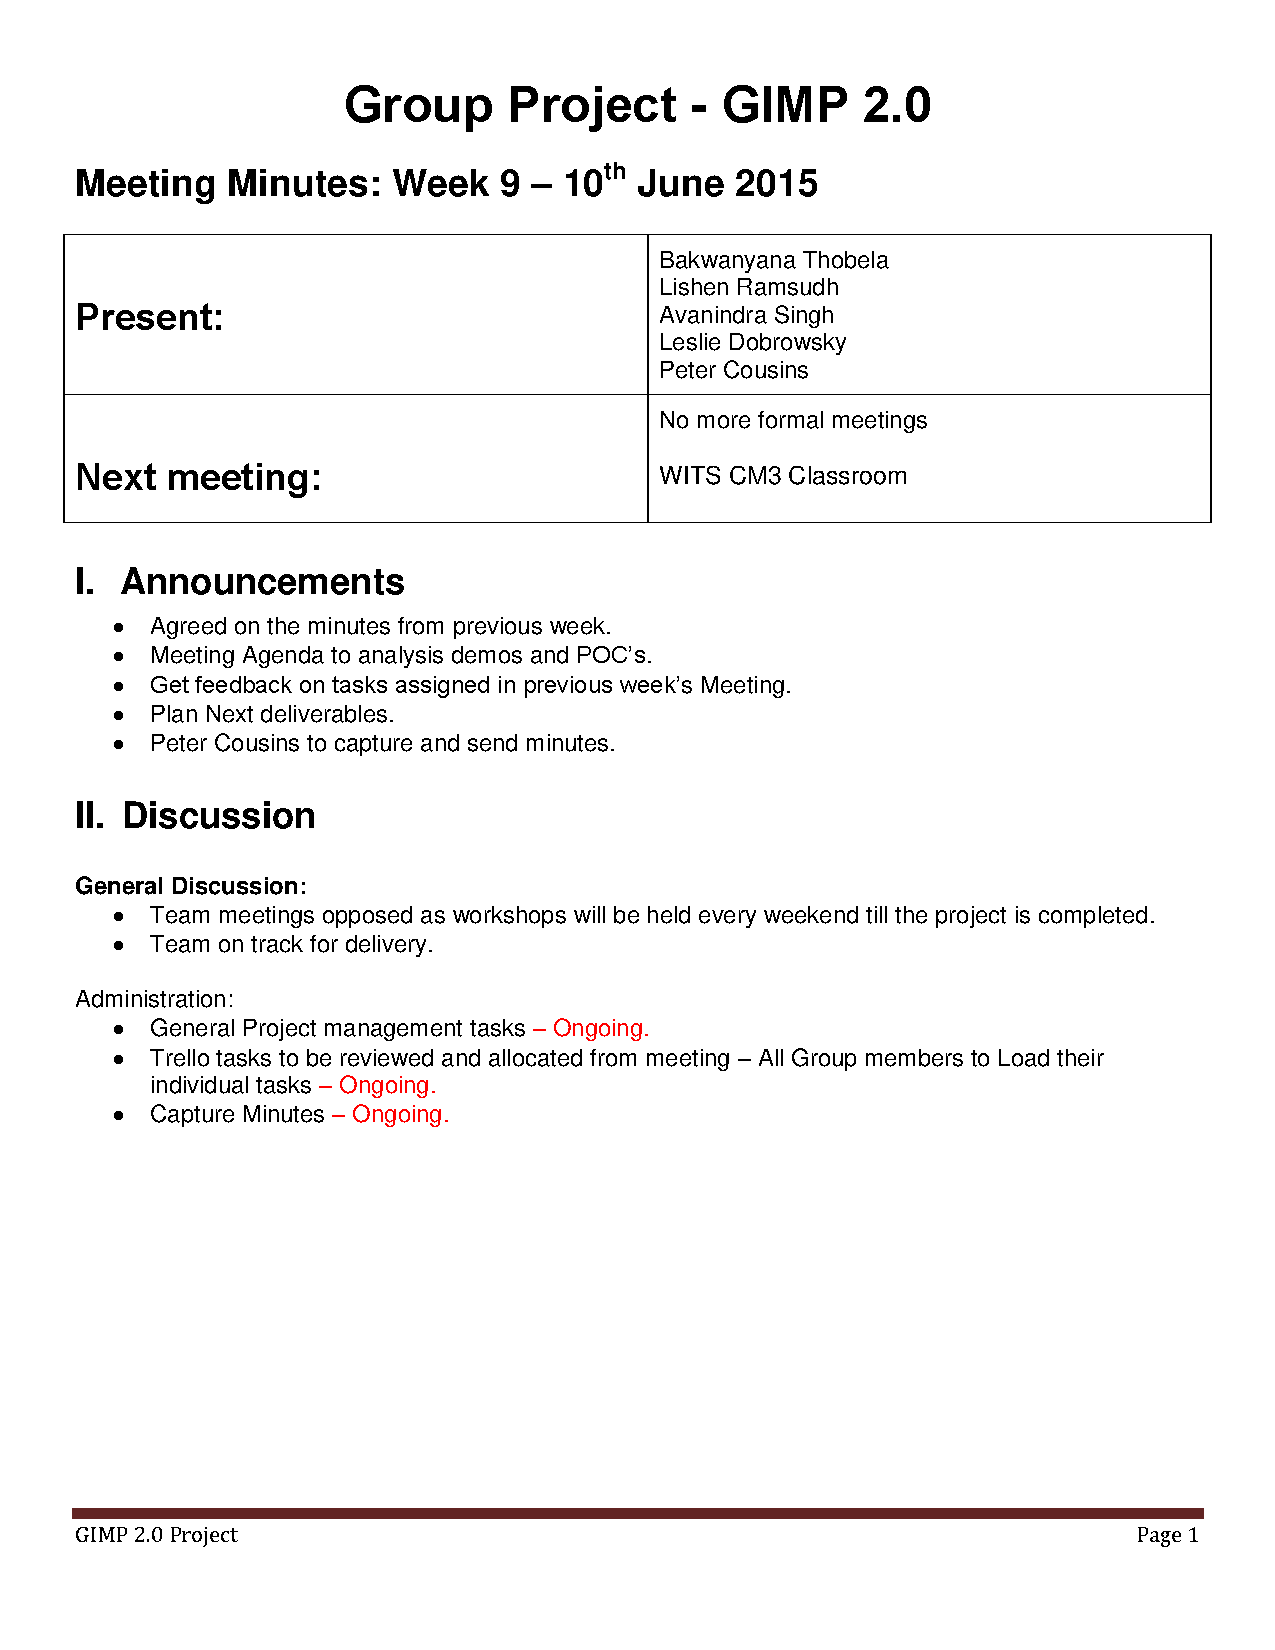
\includepdf[pages=-,scale=0.85,pagecommand={\pagestyle{fancy}}]{./sprint_planning/10Meeting.pdf}

\newpage
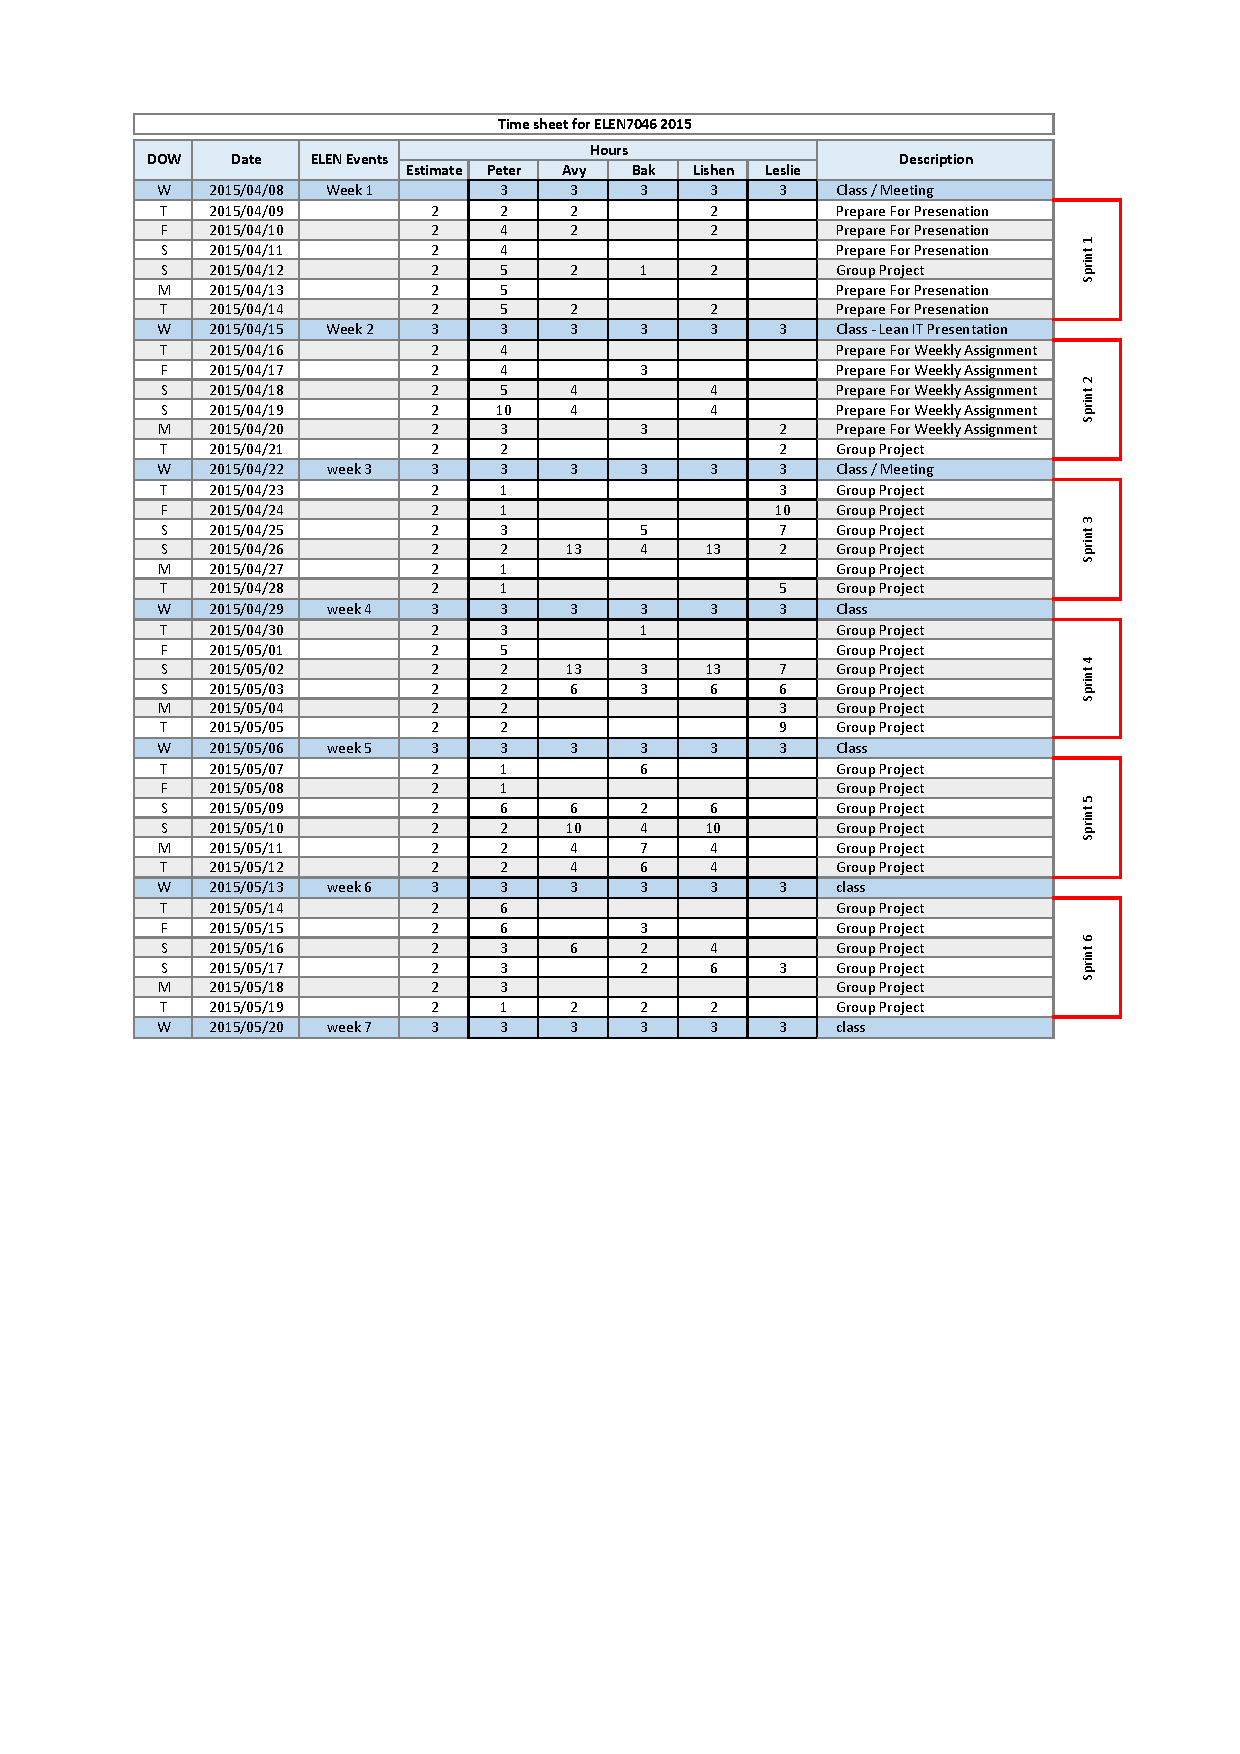
\includepdf[pages=1,scale=0.85,pagecommand=\section{Appendix H: Group Timesheet}]{./Guides/GroupTimeSheet.pdf}
\includepdf[pages=2-,scale=0.85,pagecommand={\pagestyle{fancy}}]{./Guides/GroupTimeSheet.pdf}

\newpage
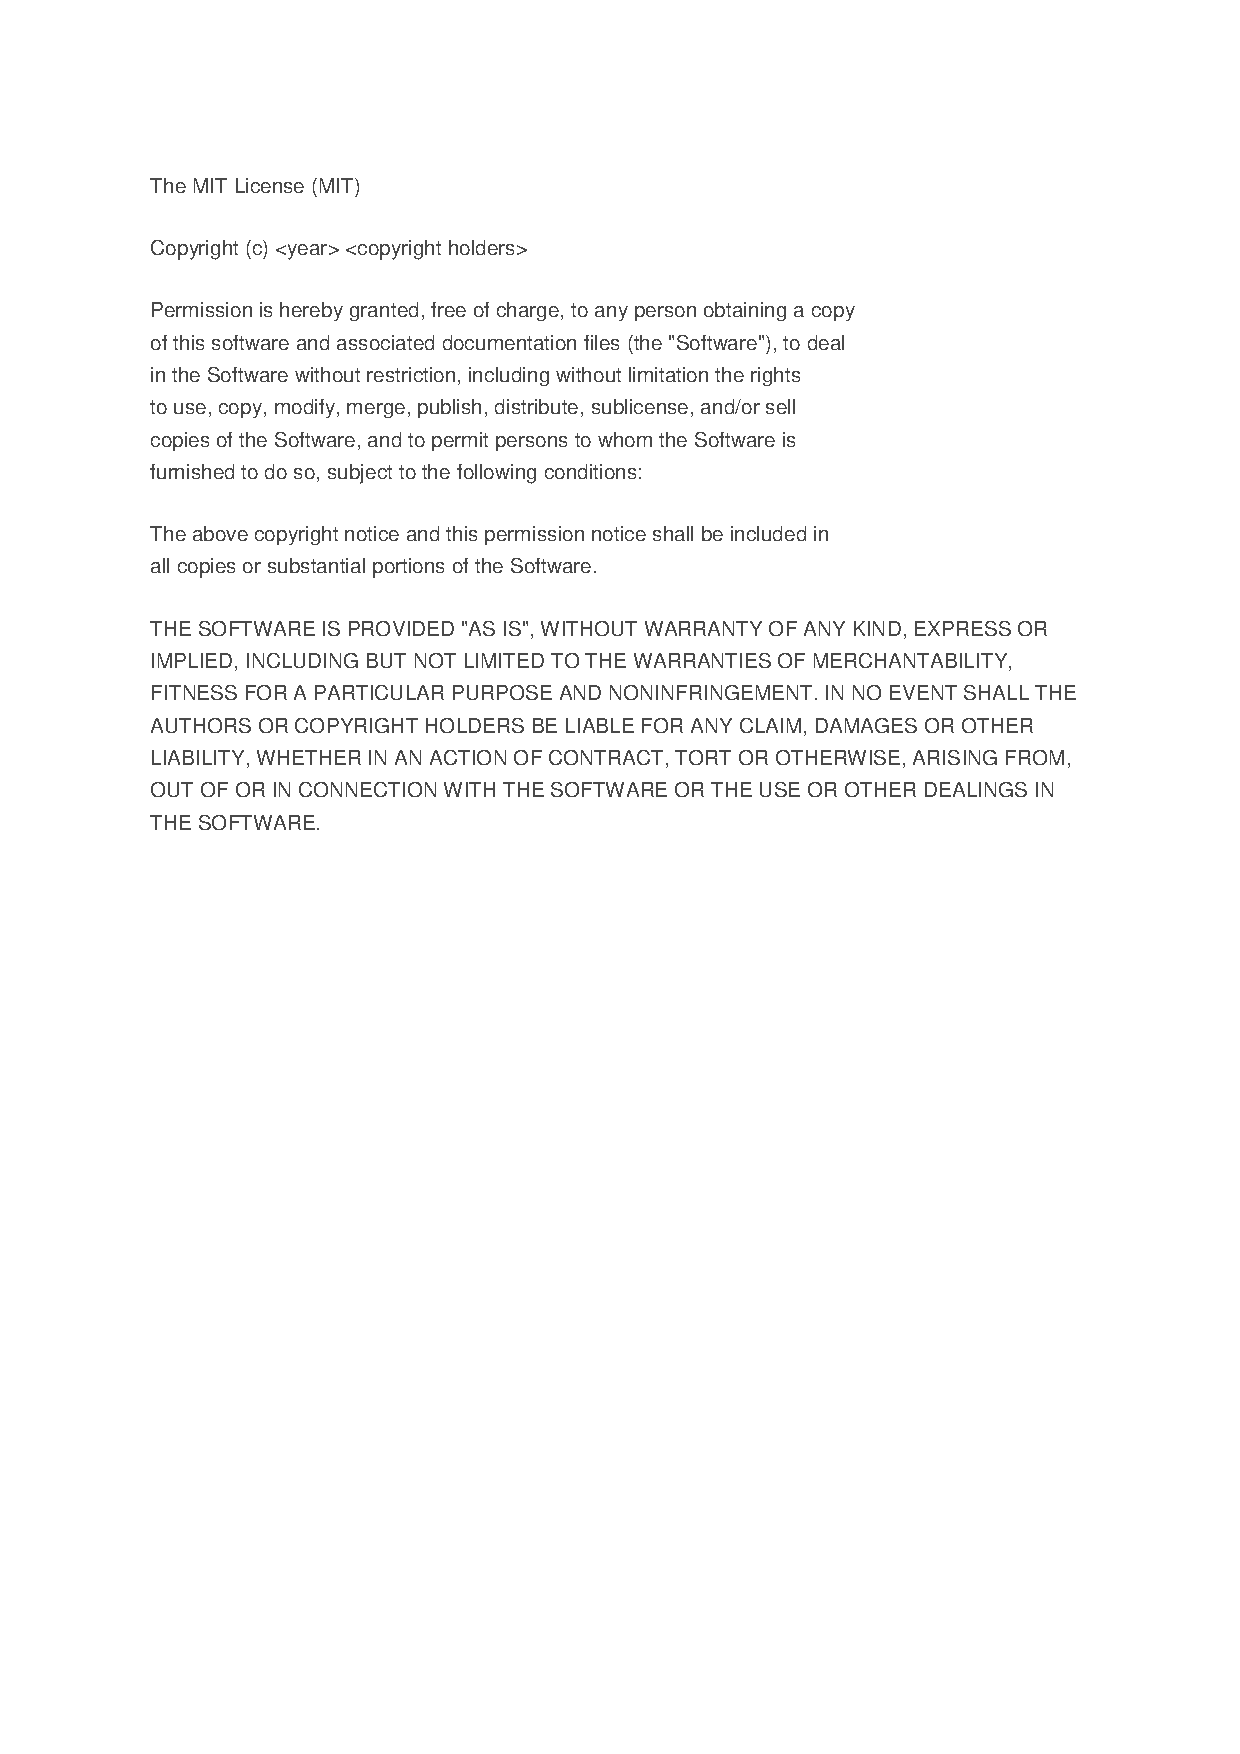
\includepdf[pages=1,pagecommand=\section{Appendix I: MIT License}]{./Guides/MIT.pdf}

\newpage
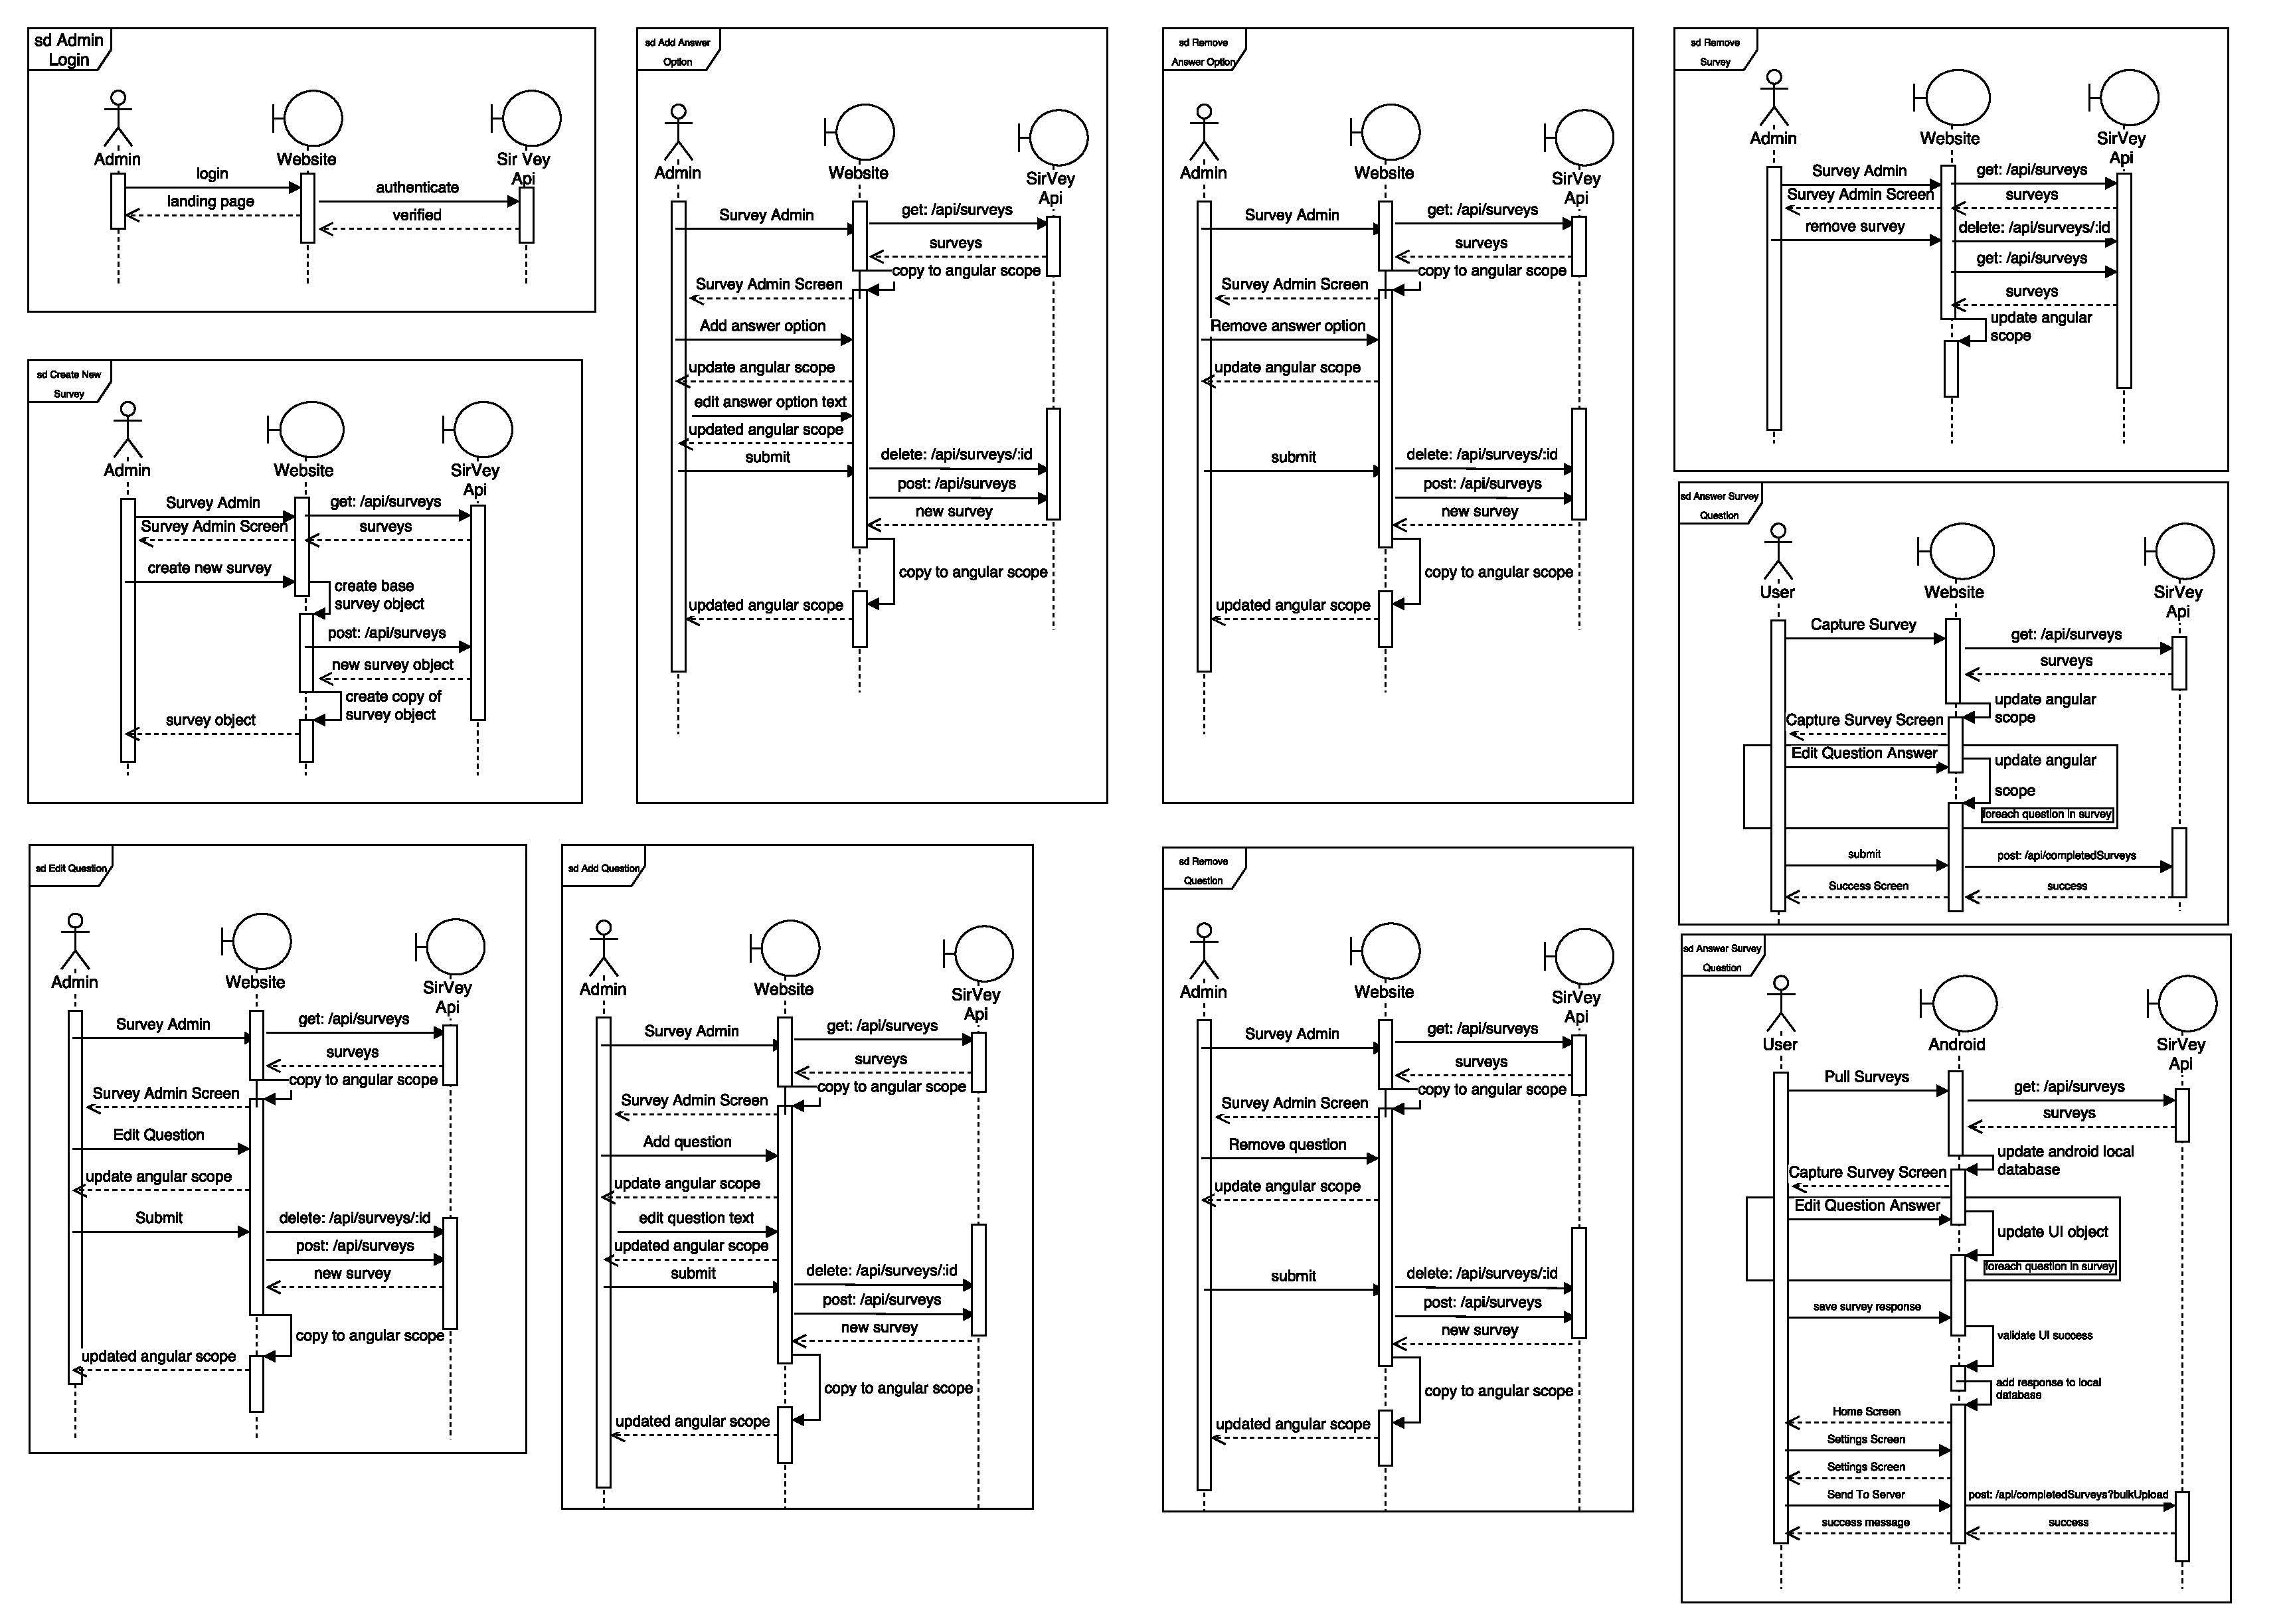
\includepdf[pages=1,pagecommand=\section{Appendix J: Sequence Diagram}]{./Guides/SirVeyApiSequenceDiagram.pdf}

\newpage
\section{Appendix K: BurnDown Chart (SCRUM)}
\begin{figure}[H]
	\center{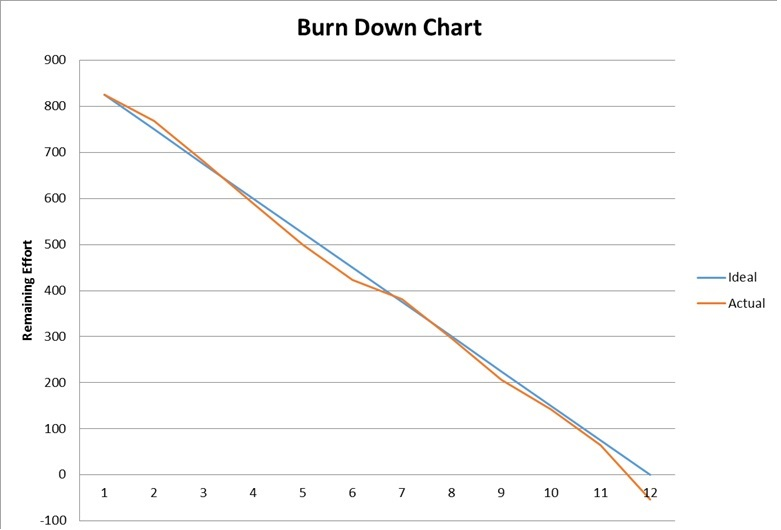
\includegraphics[width=.95\linewidth]{./images/BurnDown}} 
	\caption{Burn Down Chart for the Sirvey POC.} 
	\label{fig:BurnDown}
\end{figure}


\end{document}

% Appendix

%   A - Requirements Engineering Documentation 
% 	B - Use case diagrams
%   C - Sprint Planning / Project Planning
%   D - Dev User Guide
%   E - User Training Guide
%   F - Report Demo / Example
%   G - Meeting Minutes
%   H - Group Timesheets
%   I - Licenses
%	J - Api Design
% 	K - Burn Down Chart
